%no borrar PREAMBULO
\documentclass[12pt]{article}

\usepackage[top=3.5 cm, bottom=2.5  cm, left=3 cm, right=3 cm]{geometry}
\usepackage{fancyhdr}
\pagestyle{fancy}

\usepackage[hidelinks]{hyperref} %esta opción saca las cajas de colores de los hiperlinks

\fancyfoot[C]{\thepage }  %numera las páginas

\usepackage[utf8]{inputenc}

\usepackage{amsmath,amsfonts,amssymb}
\usepackage{xcolor}
\usepackage{fancyvrb}
\newcommand\verbbf[1]{\textcolor[rgb]{0,0,1}}%comando para colorear el texto en verbatim

%\linespread{1} %por si queremos achicar el espacio entre lineas

\usepackage{tabularx,booktabs}
\usepackage{graphicx}
\usepackage{float} %para que las figuras puedan ponerse en cualquier lado

\usepackage{subcaption}
\usepackage{layout}
\usepackage{multicol}  %para escribir en columnnas 
\usepackage{float}
\usepackage{textcomp}
\usepackage{natbib}
\usepackage{tikz}
\usepackage{multirow} %para cambiar el alto de una fila en una tabla
\tikzset{
  connect/.style = { dashed, gray }
}
\usepackage{pgfplots}
\pgfplotsset{compat=1.8}
\usepackage[english ,spanish]{babel}
\usepackage{latexsym}
\usepackage{verbatim}

%\usepackage{alltt}
\usepackage{indentfirst}

\usepackage{fancybox, calc} 

\usepackage[flushmargin]{footmisc} %para alinear las notas de página

\usepackage{url}
\usepackage{advdate}
\usepackage{wrapfig}
\usepackage{amsthm}
\usepackage[inline]{enumitem} %para hacer listas en una linea, los mismos comandos con *
\newtheorem*{myteo}{Teorema} % la * es para no numerarlos
\newtheorem*{myexample}{Ejemplo}
\newtheorem*{myprop}{Proposición}
\newtheorem*{mylem}{Lema}
\theoremstyle{definition}
\newtheorem*{mydef}{Definición}
\newtheorem{ejer}{Ejercicio}
\newtheorem*{mydefs}{Definiciones}
%\theoremstyle{remark}
\newtheorem*{myobs}{Observación}
\newtheorem*{remark}{Importante}

\renewcommand{\baselinestretch}{1}  %interlineado

\addto\captionsspanish{%
  \renewcommand{\figurename}{Figura}%
}

\newcommand\myText[1]{\text{\scriptsize\tabular[t]{@{}l@{}}#1\endtabular}}
\addto\captionsspanish{%
  \renewcommand{\tablename}{Tabla}%
}

\def \ds {\displaystyle} %define un comando abreviado  
\def\com{“R”}

\usepackage{hyperref}%para referencias de internet con link!
\newcommand*{\fullref}[1]{\hyperref[{#1}]{ \nameref*{#1}}}
%comando \fullref para que ademas del número de capitulo, sección etc. escriba el título del capitulo, sección o lo que sea a lo que estamos haciendo referencia

\newcommand\comentario[1]{\textcolor{red}{#1}}%comentarios en el pdf

\interfootnotelinepenalty=10000 %previene que se pasen a otra página las notas de pie
\raggedbottom 
\addtolength{\topskip}{0pt plus 10pt}
\addtolength{\footnotesep}{0.1mm}

\VerbatimFootnotes%para poder usar Verbatim en las notas de pie

\begin{document}

\fancyhf{}
\pagestyle{fancy}
\lhead{Departamento de Matem\'{a}tica\\Universidad Nacional del Comahue}
\rhead{Matem\'{a}tica 1\\ Licenciatura en Ciencias Biol\'{o}gicas}

%HASTA ACA 

\begin{centering}
\Large{\textbf{Trabajo Práctico N° 2}}\\
\large{\textbf{Relaciones y Funciones}}\\
\end{centering}

\vspace{1cm}

%Definicion de par ordenado
\fbox{ \parbox{0.98\linewidth}{
\noindent
\begin{mydef}  \textbf{Par ordenado.}
\noindent

Un par ordenado es una pareja de objetos matemáticos, en la que se distingue un primer elemento y un segundo elemento. El par ordenado cuyo primer elemento es $a$ y cuyo segundo elemento es $b$ se denota como $(a, b)$.\\ 
Es importante aclarar que un par ordenado no es un conjunto, sino un objeto donde están definidos dos elementos que lo componen ($a$ y $b$) y un orden entre esos elementos, mientras que en un conjunto se indican sus elementos y no hay indicaciones de orden.\\
En este sentido, debemos notar que si se trata de pares ordenados, $(a, b) \neq (b, a)$, mientras que si se trata de conjuntos, los conjuntos $\{ a, b  \}$ y $\{ b,a \}$ son iguales.  Dos pares ordenados $(a, b)$ y $(c, d)$ son iguales si y sólo si coinciden respectivamente sus elementos, es decir, debe ser $a = c$ y $b = d$.

\end{mydef}
}}

\vspace{0.5 cm}

%Definicion de producto cartesiano
\fbox{ \parbox{0.98\linewidth}{
\noindent
\begin{mydef}  \textbf{Producto cartesiano}\\
\noindent
El producto cartesiano de los conjuntos $A$ y $B$ será un nuevo conjunto que denominaremos $A \times B$ formado por todos los pares ordenados posibles formados con los elementos de $A$ y $B$, donde el primer elemento pertenece a $A$ y el segundo elemento pertenece a $B$.  En símbolos: \\
\setlength\itemsep{0em}
\begin{equation*}
  A \times B = \{ (a,b) / a \in A \text{ y } b \in B)
\end{equation*}
\end{mydef}
}}

\begin{enumerate}
%1
\item Tomar los conjuntos siguientes, dar el producto cartesiano por extensión y elegir alguna forma de representación gráfica:\\

$A = \{  \text{Norte, Sur, Este, Oeste}\}, B = \{ \text{Lunes, Miércoles, Jueves, Viernes}\}$

%2
\item Considerar los conjuntos siguientes y graficar el producto cartesiano en el plano $\mathbb{R}^2$, y escribir las condiciones que deben cumplir los pares $(x,y)$ para pertenecer al mismo. 
\begin{enumerate} [leftmargin=2cm]
\item $A = \{ x \in \mathbb{R} / x \geq 2 \text{ y } x \leq 5 \} $ y $B = \{ x \in \mathbb{R} / x < 4\}$ 
\item  $A =  \{ x \in \mathbb{R} / x \geq 4\}$ y $B = \{ x \in \mathbb{R} / x < 5\}$ 
\item  $A = \{ x \in \mathbb{R} / x > 2 \text{ y } x \leq 6 \}$ y $B = \{ x \in \mathbb{R} / x \geq 3 \text{ y } x \leq 6 \}$ 
\end{enumerate}


%Definicion de relaciones
\fbox{ \parbox{0.98\linewidth}{
\noindent
\begin{mydef}  \textbf{Relaciones.}\\
\noindent
Una relación entre el conjunto $A$ y el conjunto $B$ es un subconjunto del producto cartesiano $A \times B$. Es decir, es una aplicación que vincula algunos elementos de $A$ (eventualmente todos) con algunos elementos de $B$ (eventualmente todos). \\
En una relación, al conjunto $A$ lo llamaremos  \textbf{conjunto de partida}, y a $B$,  \textbf{conjunto de llegada}. 
\end{mydef}
}}

\vspace{0.5 cm}

%Definicion de producto cartesiano
\fbox{ \parbox{0.98\linewidth}{
\noindent
\begin{mydef}  \textbf{Dominio e imagen.}\\
\noindent
Llamaremos \textbf{dominio} de la relación al subconjunto del conjunto de partida constituido por los elementos que tienen relación con elementos del conjunto de llegada.  También, llamaremos \textbf{imagen} (o rango) al subconjunto del conjunto de llegada constituido por los elementos que están relacionados con elementos del conjunto de partida. \\
Para el elemento $x$ del dominio al que corresponde el elemento $y$ de la imagen, decimos que $y$ es \textbf{la imagen} de $x$ mediante esta relación, y que $x$ es \textbf{la preimagen} de $y$ por esta relación. En ocasiones suele escribirse $x R y$.
\end{mydef}
}}


\begin{myexample}
Tomemos el conjunto de las personas de Bariloche como conjunto de partida y números enteros positivos de siete cifras que empiezan con 4  (por ejemplo 4439821) como conjunto de llegada.  Consideremos la relación “$x$ (una persona) \textit{tiene como número de teléfono fijo al número} $y$ (número de siete cifras)” Seguramente habrá alguna persona que no tenga un teléfono fijo. El dominio entonces no coincide con el conjunto de partida, sino que estará constituido sólo por las personas que tienen teléfono fijo (cuál  número y cuántas líneas es otro cantar). También es cierto que no todo número de siete cifras empezado en 4 califica para número de teléfono. Más de una vez habremos llamado a alguien (y metido mal el dedo) y habremos escuchado a la chica de Telefónica que nos dice “el número solicitado no corresponde a un abonado en servicio”. Es decir, no todo número es el número de alguien. Es decir, dentro del conjunto de números enteros positivos de siete cifras que empiezan con 4, sólo algunos son efectivamente números de teléfonos de alguien. La imagen entonces no coincide con el conjunto de llegada, sino que estará constituida sólo por los números de siete cifras empezados con 4 que corresponden a un número de teléfono de alguna persona.
\end{myexample}

%3
\item Considerar la relación R: “es el DNI de”. Proponer un conjunto de partida y un conjunto de llegada. Escribir el dominio y la imagen.

%4
\item Lo mismo para la relación R: “tiene el número de DNI”.

%6
\item En cada uno de los casos anteriores, ¿es posible que haya situaciones como las del dibujo siguiente? Ejemplificar
\begin{center} 
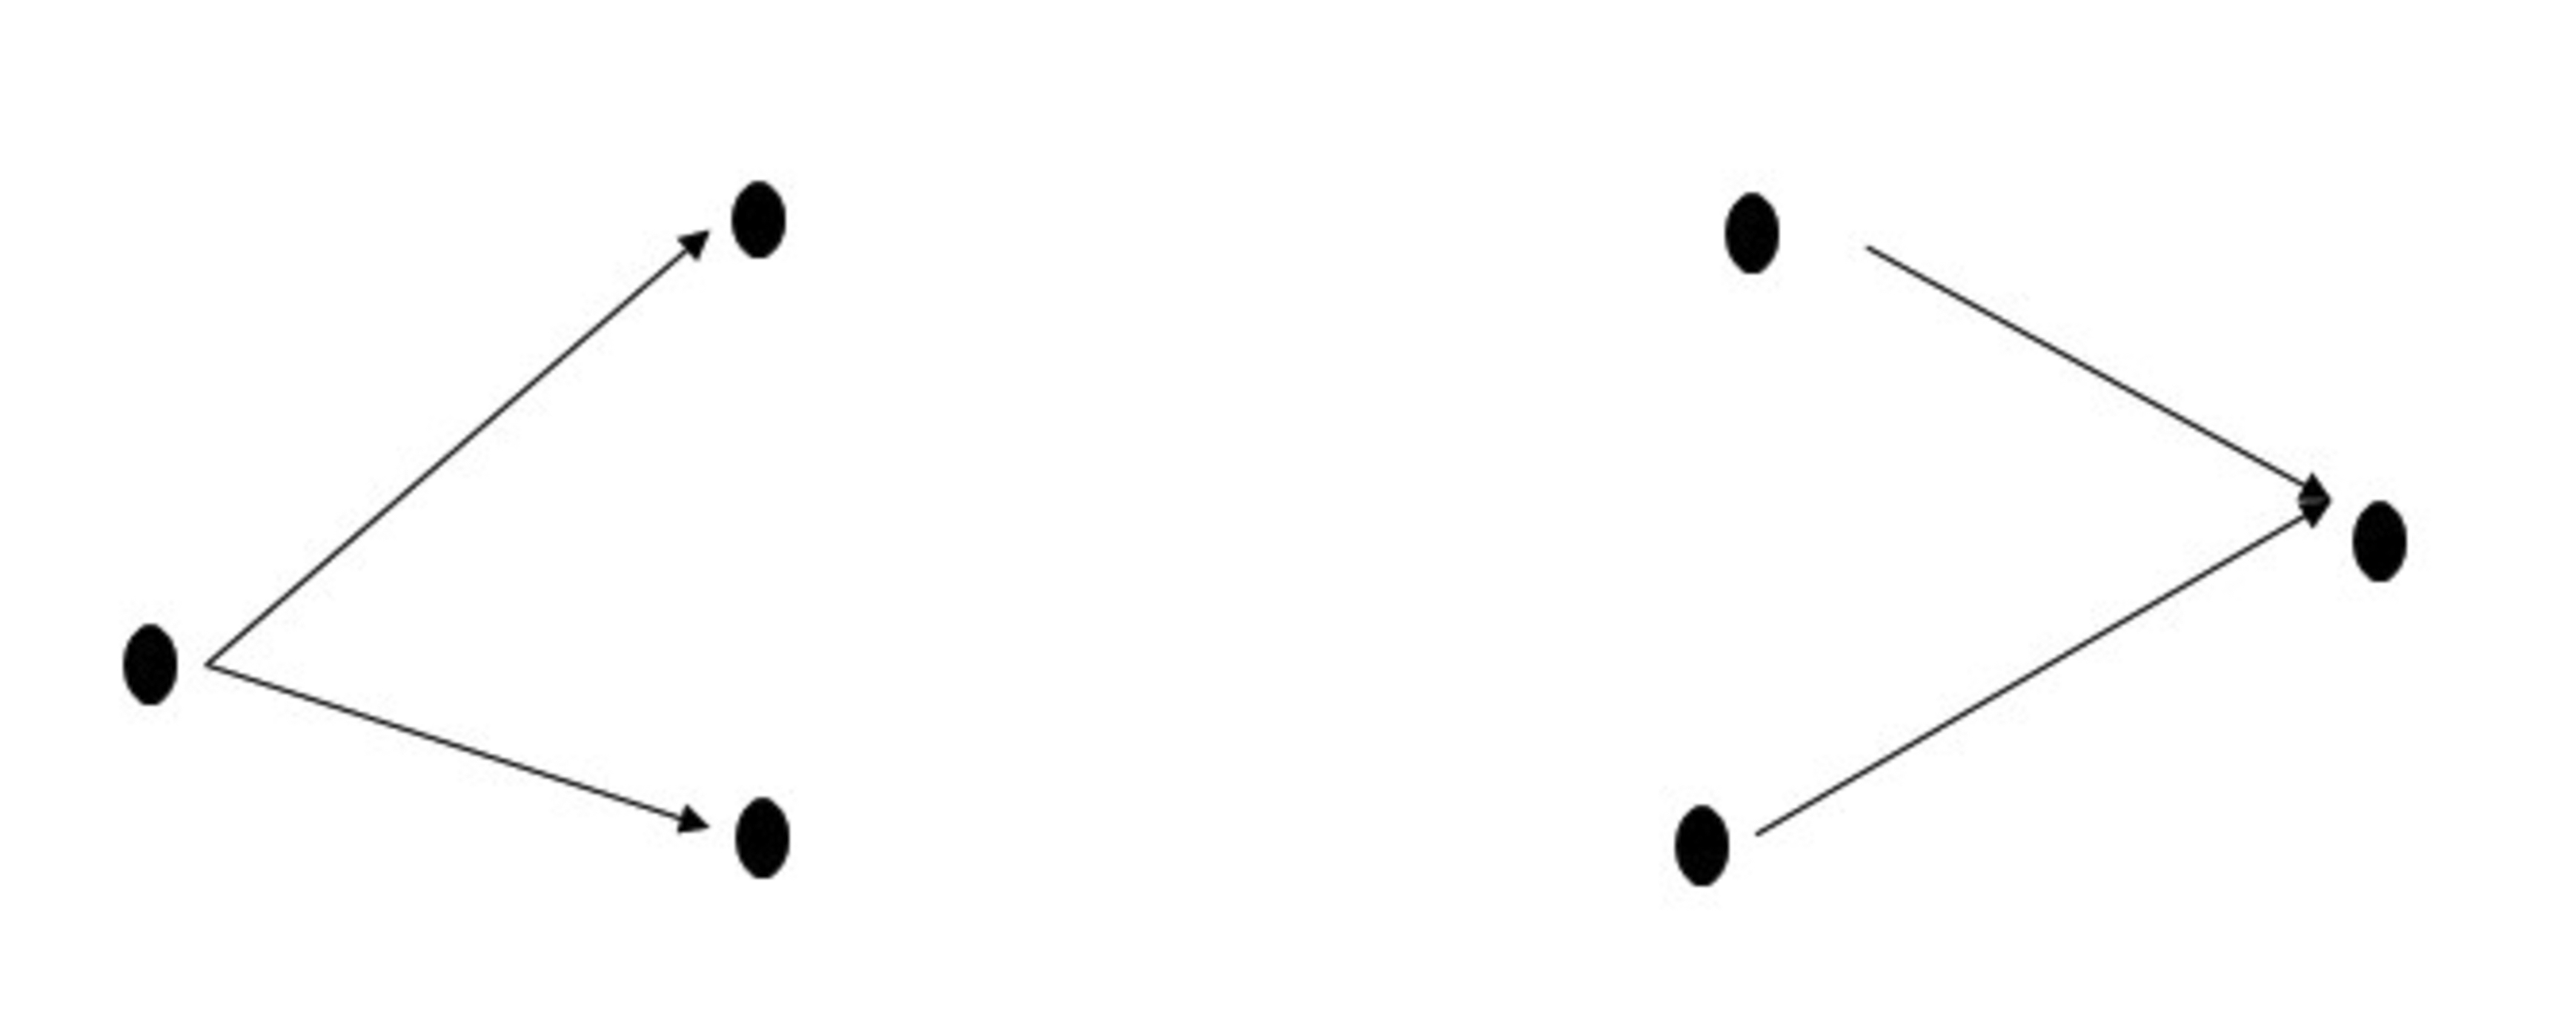
\includegraphics[width=0.5\textwidth]{tp2_fig1.jpg} 
\end{center}

Otra cosa interesante de las relaciones es la forma en que los elementos se vinculan. En el ejemplo de los teléfonos, es posible que una persona sea titular de más de una línea, con lo cual su relación en el gráfico sería algo como el dibujo de la izquierda:
\begin{center} 
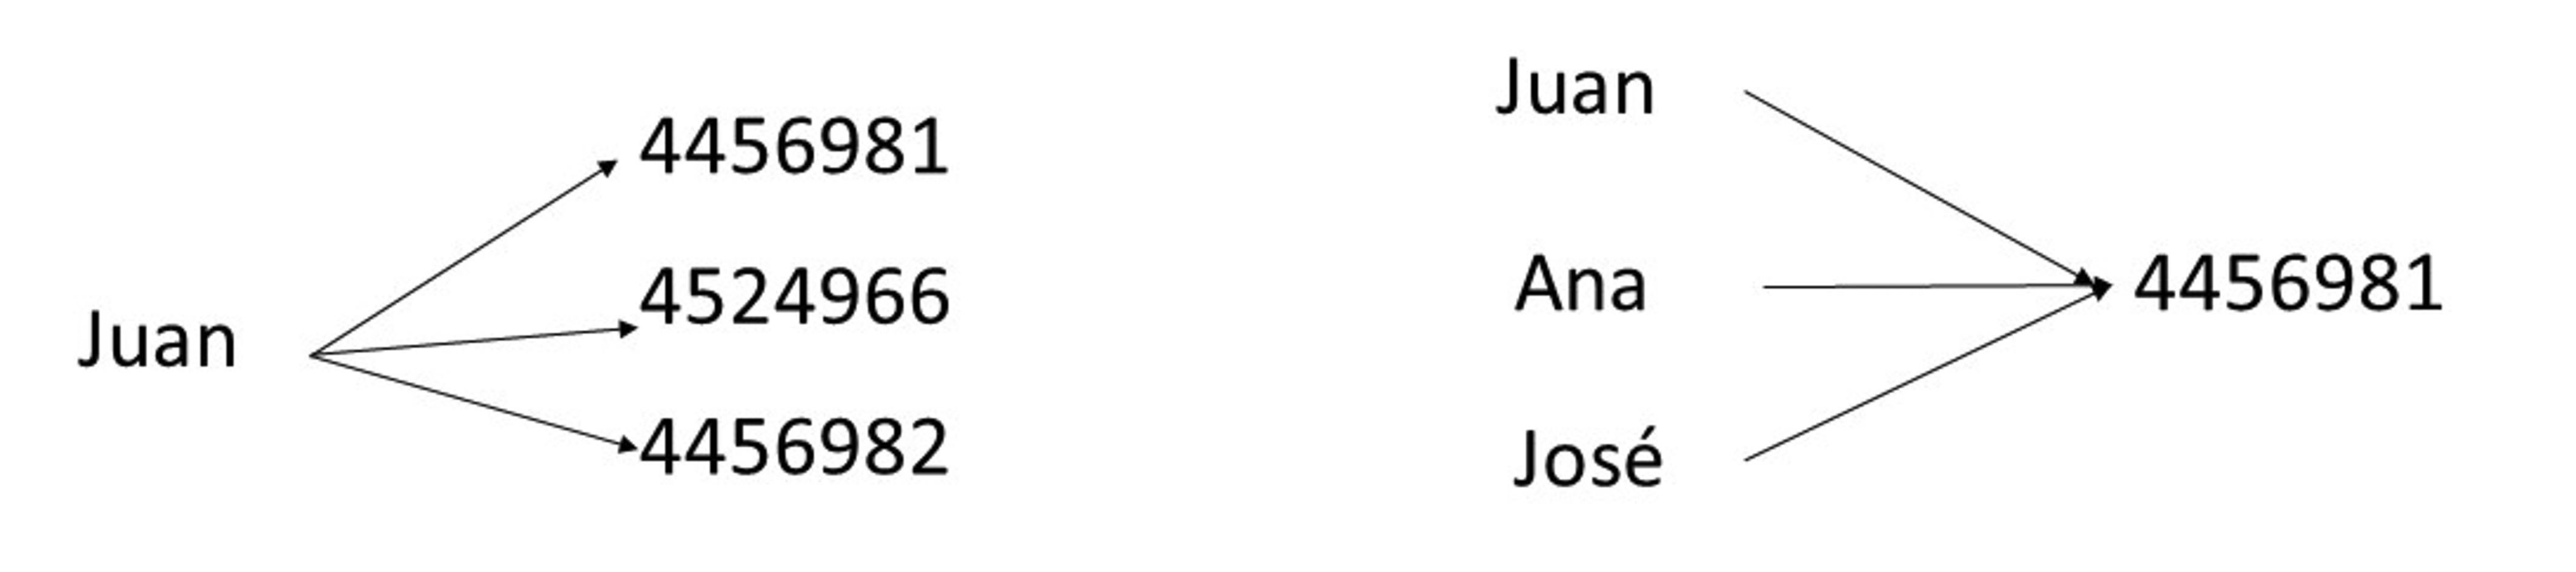
\includegraphics[width=0.7\textwidth]{tp2_fig2.jpg} 
\end{center}

Y también puede ocurrir que un número de teléfono sea el mismo para varias personas, como  se ve en el diagrama de la derecha. También es posible que en una relación haya una correspondencia de un elemento del conjunto dominio con uno y sólo un elemento del conjunto imagen, como por ejemplo la relación R: “es el DNI de”, donde el dominio es el conjunto de números que son números de DNI y la imagen un conjunto de personas. Cada DNI corresponde a una persona y esa persona es única. Es decir, no puede pasar ni lo del diagrama de la izquierda ni lo del de la derecha. En este caso, decimos que se establece una relación \textbf{uno a uno} entre los elementos de ambos conjuntos. \\

En muchas ocasiones nos enfrentamos con relaciones entre dos magnitudes en las cuales el valor de una de ellas depende del valor de la otra. Por ejemplo, si vamos a comprar papas, lo que paguemos en la verdulería (costo) depende de la cantidad de papas que compremos.  O por ejemplo, el costo de una encomienda depende de su peso. Hay una \textbf{variable dependiente} de otra (que podemos llamar \textbf{independiente}). Estas relaciones pueden tener diversas formas de representación: gráfica, por medio de una fórmula, o por medio de una tabla de valores, donde se muestren los valores que adopta una variable de acuerdo al valor que adopta la otra.\\

Pongamos por ejemplo el gráfico siguiente, que representa la posición de un ciclista en función del tiempo respecto de un punto de partida (en el que ubicaremos el 0). En el eje horizontal está representado el tiempo (en minutos), y en el eje vertical la posición del ciclista (en metros desde el punto de partida), denotada como $p(m)$. 
\begin{center} 
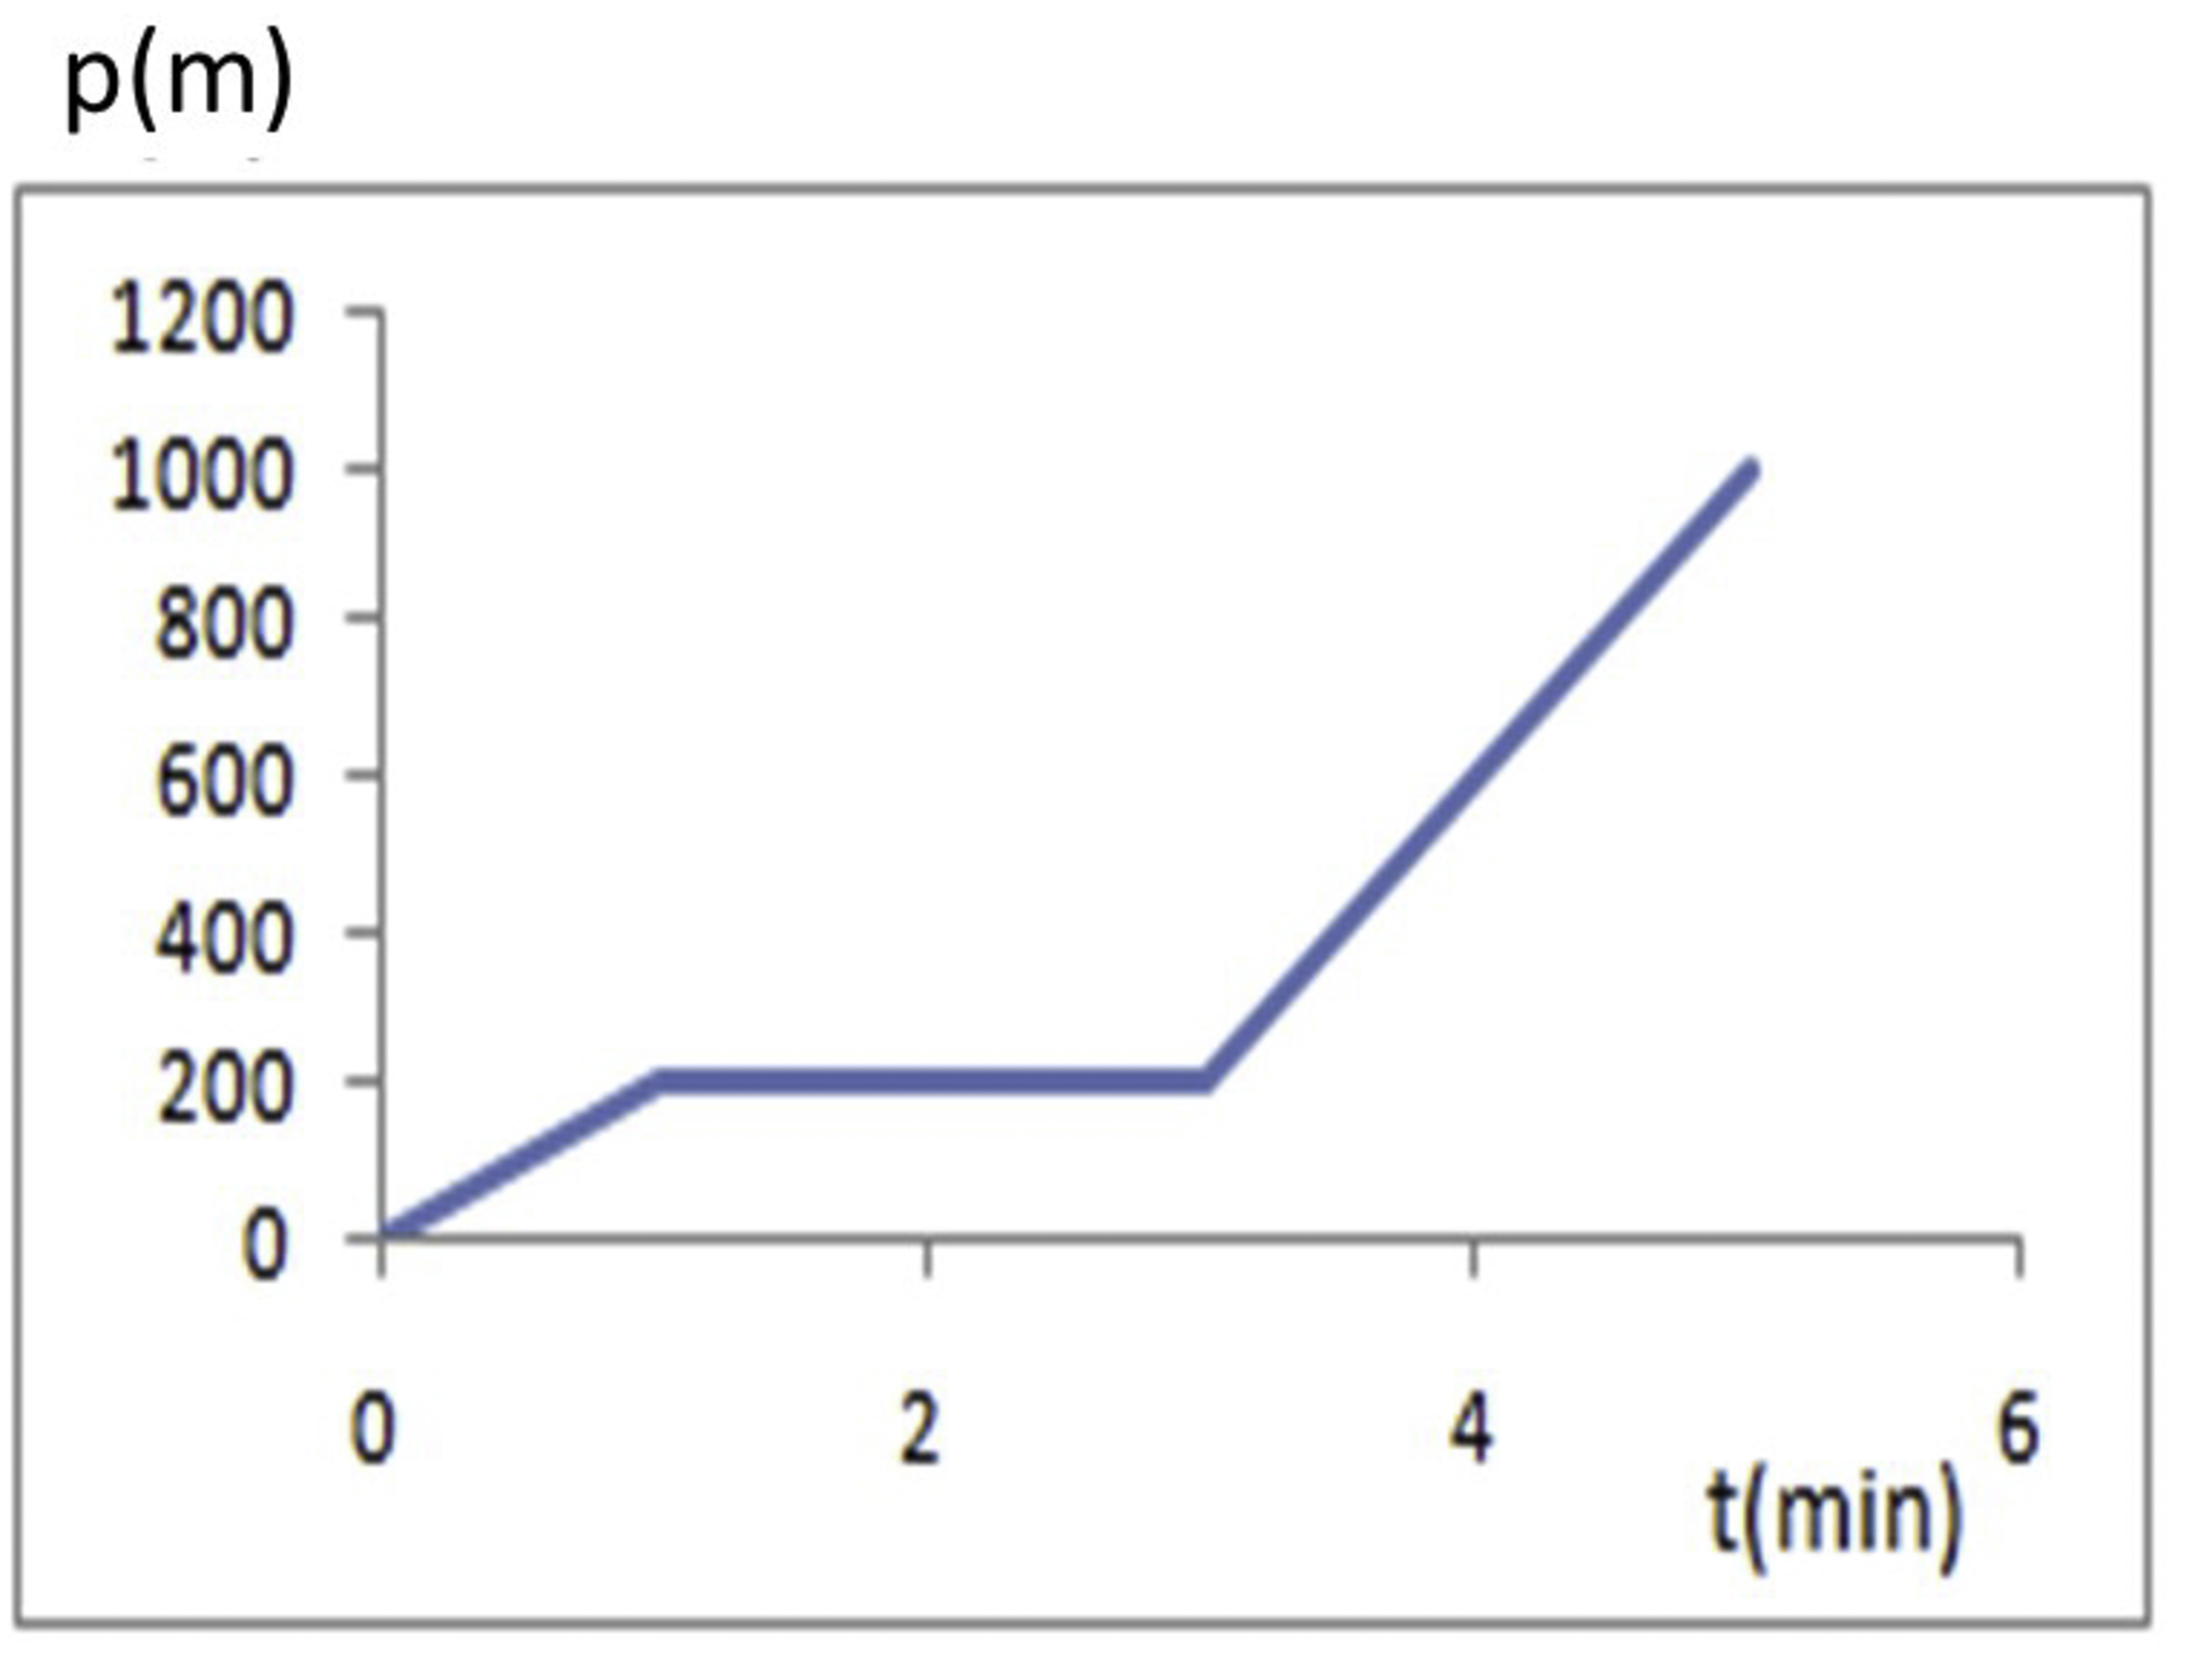
\includegraphics[width=0.4\textwidth]{tp2_fig5.jpg} 
\end{center}
Vemos que a cada tiempo corresponde un único valor de distancia, es decir, a cada instante de tiempo que tomemos entre $0$ y $5$ minutos, la distancia que recorrió el ciclista es única. La variable tiempo, es la que llamamos variable independiente, entendiendo por eso que podemos elegir libremente el tiempo para el cual queremos saber cuál es la distancia recorrida por el ciclista. La variable distancia es la que llamamos variable dependiente, entendiendo por eso que la distancia que haya recorrido el ciclista depende del tiempo que haya transcurrido desde su partida.\\ 

La variable independiente se grafica en el eje horizontal, que llamamos  \textbf{eje de abscisas}, y a la variable dependiente en el eje vertical, que llamamos  \textbf{eje de ordenadas}.\\ 

La particularidad de esta relación y de las relaciones recién mencionadas es que para un determinado valor de la variable independiente, el valor de la otra variable es único.  A este tipo de relaciones donde a cada valor de la variable independiente corresponde un único valor de la variable dependiente, se las llama  \textbf{funciones}. Y decimos que la variable dependiente es función de la variable independiente.\\

\fbox{ \parbox{0.98\linewidth}{
\noindent
Para que una relación entre dos variables sea una función, a cada valor de la variable independiente (cada valor del conjunto de partida) tiene que corresponder un único valor de la variable dependiente, (un único valor del conjunto de llegada).\\
}}
\vspace{0.5 cm}

%Definicion de función
\fbox{ \parbox{0.98\linewidth}{
\noindent
\begin{mydef}  \textbf{Función.}\\
\noindent
Una relación $f:A \rightarrow B$ es una \textbf{función} si a cada elemento del conjunto $A$ se tiene asociado un único elemento del conjunto $B$.\\
Al conjunto formado por todos los elementos de $A$ que tienen una imagen se lo denomina  \textbf{dominio} de la función $f$, y al conjunto formado por todos los elementos de $B$ que son imagen de algún elemento del dominio se lo llama  \textbf{imagen} (o rango). \\
Si  llamamos $x$ a un elemento genérico del conjunto dominio, e $y$ al elemento que $f$ asigna a $x$, escribimos $y = f(x)$, que significa que el elemento $y$ está asociado al elemento $x$ por medio de la función $f$, o dicho de otra manera, $y$ es \textbf{la imagen} de $x$ por $f$. 
\end{mydef}
}}

%7
\item Para las relaciones vistas en el apartado anterior, identificar cuáles son funciones, cuál es su conjunto dominio y cuál su conjunto imagen.

%8
\item Proponer relaciones que sean funciones y relaciones que no lo sean, explicando las razones por las cuales lo son o no, y mostrando en caso de serlo, sus conjuntos dominio e imagen.

\fbox{ \parbox{0.98\linewidth}{
\noindent
Para varias de las actividades que vamos a desarrollar a continuación sería ideal disponer del software \textit{Graph 4.3}. Es un software libre para graficar funciones, se puede bajar de:
\begin{center} 
\textcolor{blue}{www.padowan.dk/graph}
\end{center}
Es de muy fácil manejo, sencillo de instalar y muy versátil.
}}
\vspace{0.2 cm}

%9
\item Considerar un sistema de ejes cartesianos en el plano. Ubicar en él los siguientes puntos: $(-1,1)$;  $(0,2)$;  $(3,0)$;  $(-2,0)$; $(0,\frac{1}{2})$;  $(-2,-3)$

%10
\item Escribir las coordenadas de los puntos señalados en el gráfico:
\begin{center} 
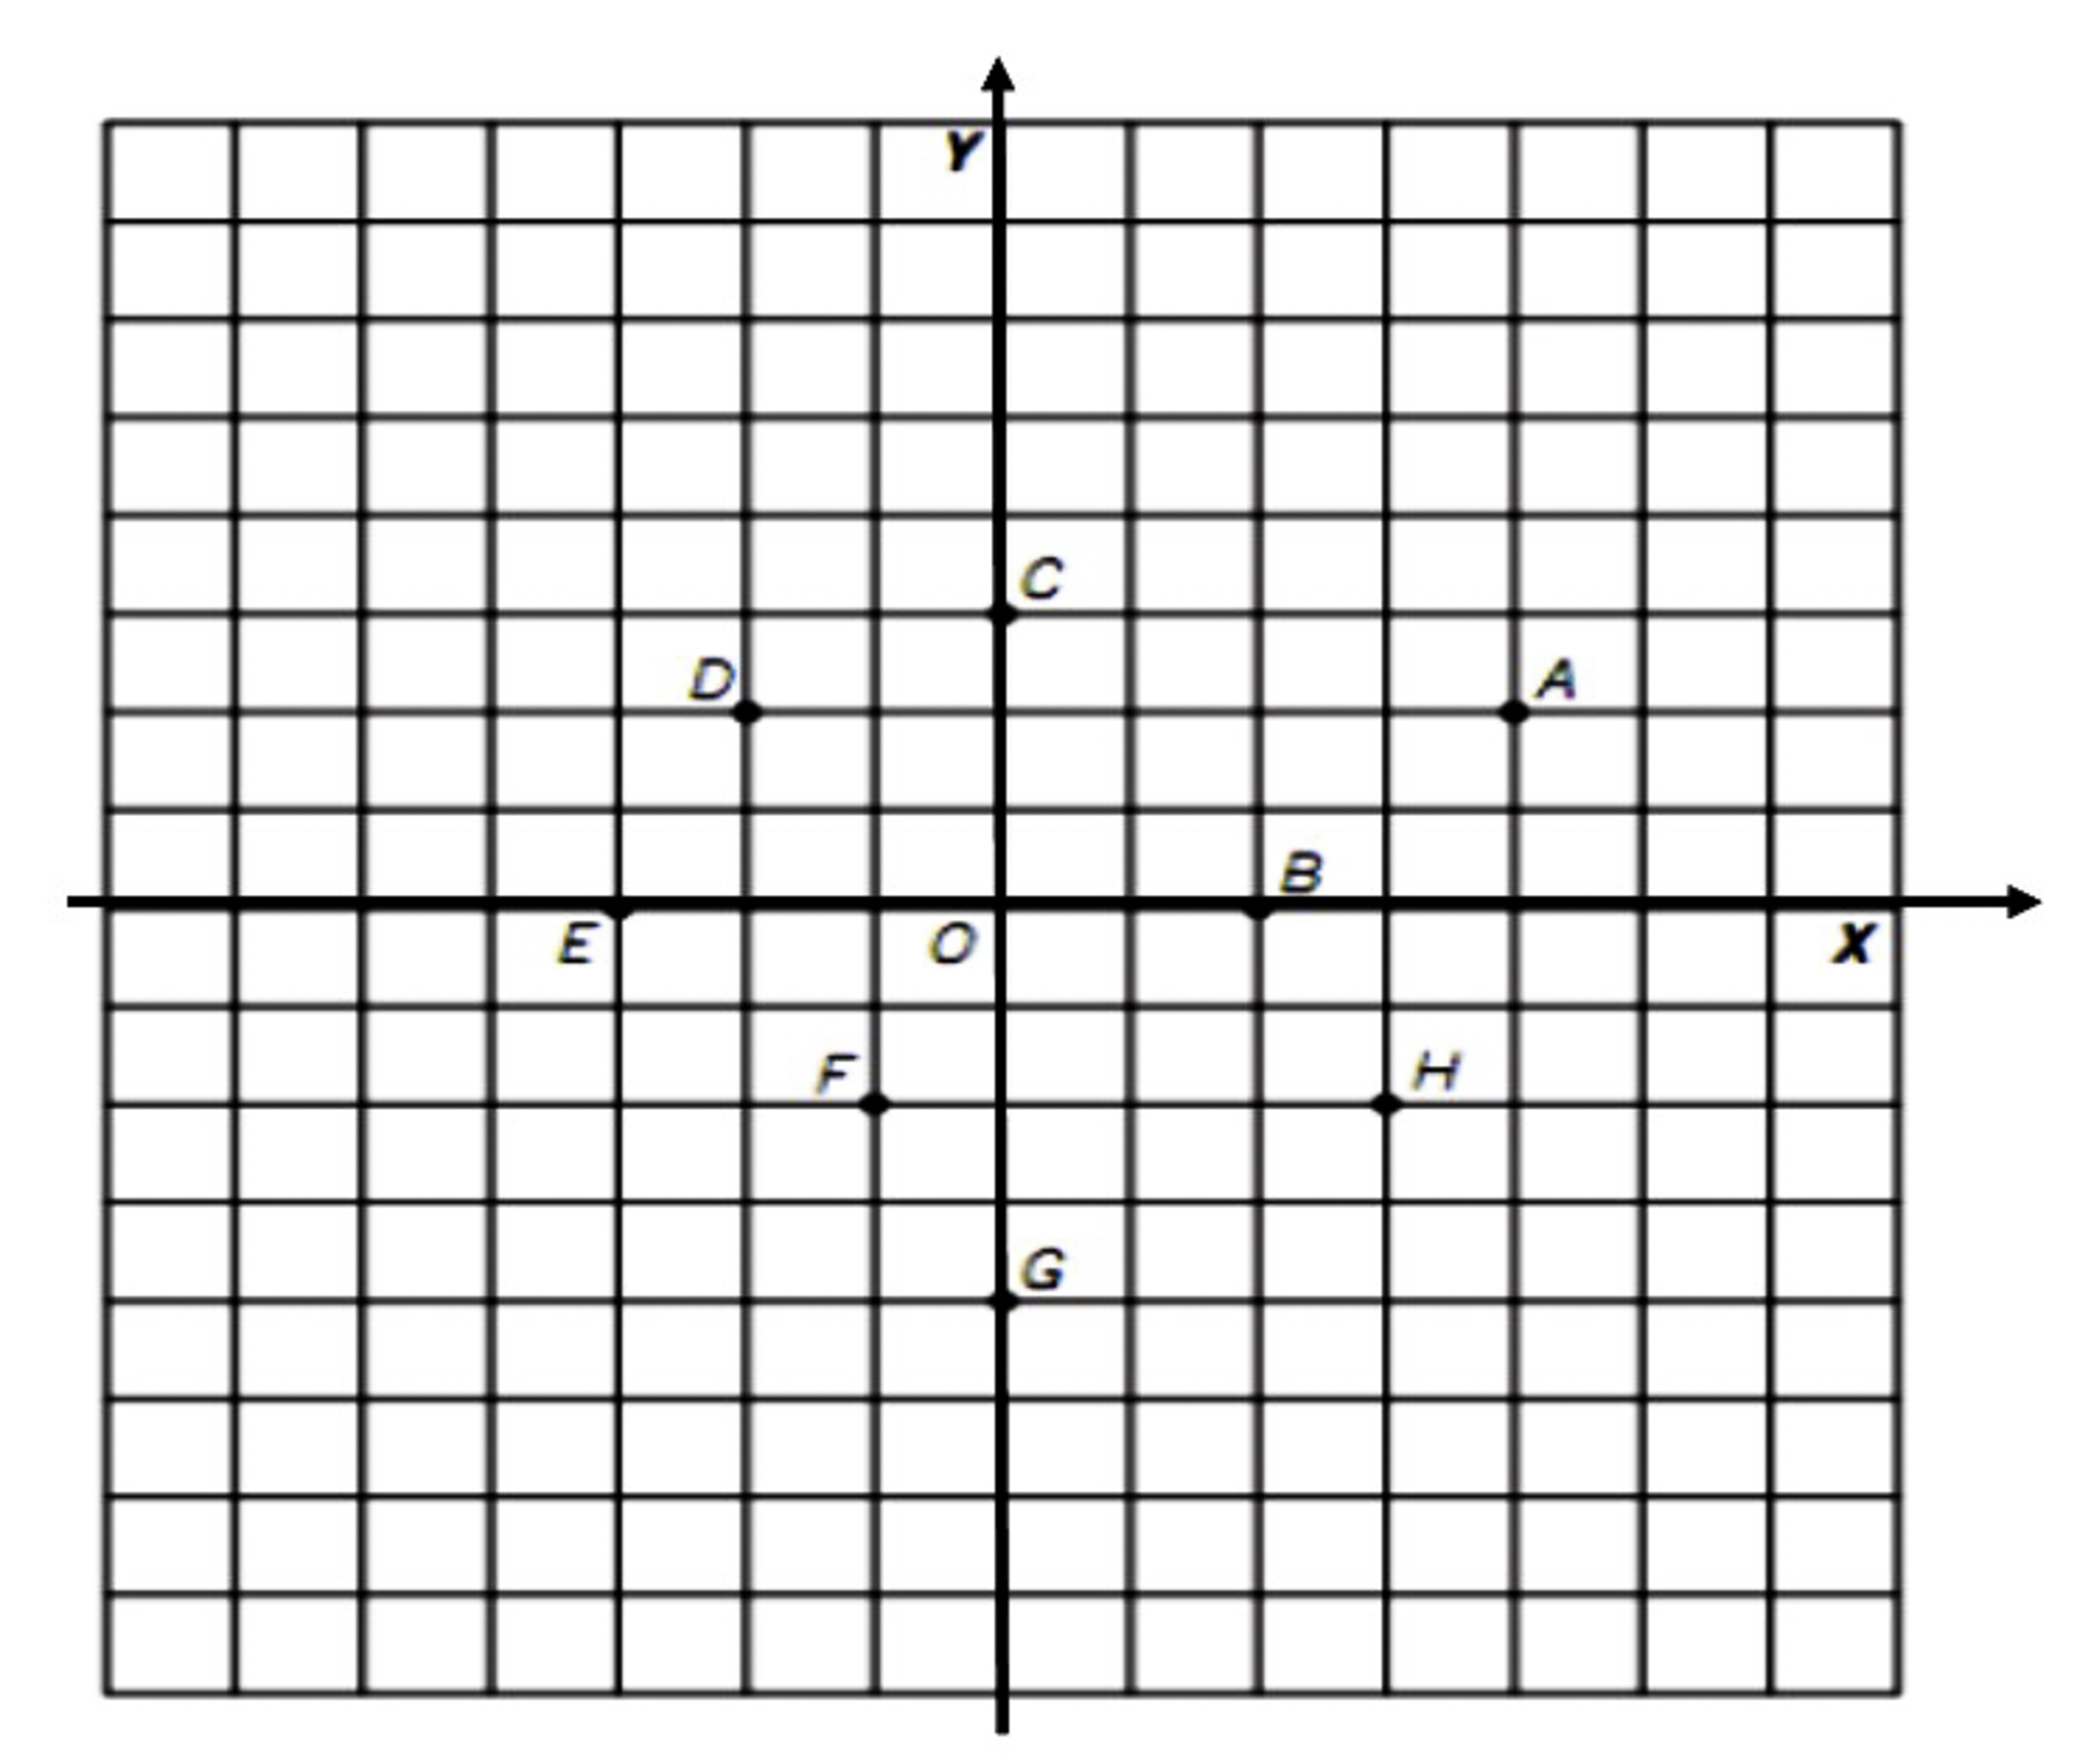
\includegraphics[width=0.4\textwidth]{tp2_fig3.jpg} 
\end{center}

%11
\item Marcar en el plano cartesiano los conjuntos de puntos que cumplen las siguientes condiciones:
\begin{multicols}{4}
\begin{enumerate} [leftmargin=2cm]
\item $x = 0$ 
\item  $x > 0$
\item $y = 0$ 
\item  $y > 0$
\item  $y < 0$ 
\item $y \geq 1$
\item  $x < 5$
\item  $x > -1$
\end{enumerate}
\end{multicols}


%12
\item No siempre una relación es una función. Supongamos que estamos estudiando la memoria de las personas mediante un test que asigna un puntaje, y que queremos ver cuál es la relación entre el puntaje obtenido en el test y la edad de la persona. Podríamos obtener lo siguiente, visto en un gráfico o en una tabla:
\begin{center} 
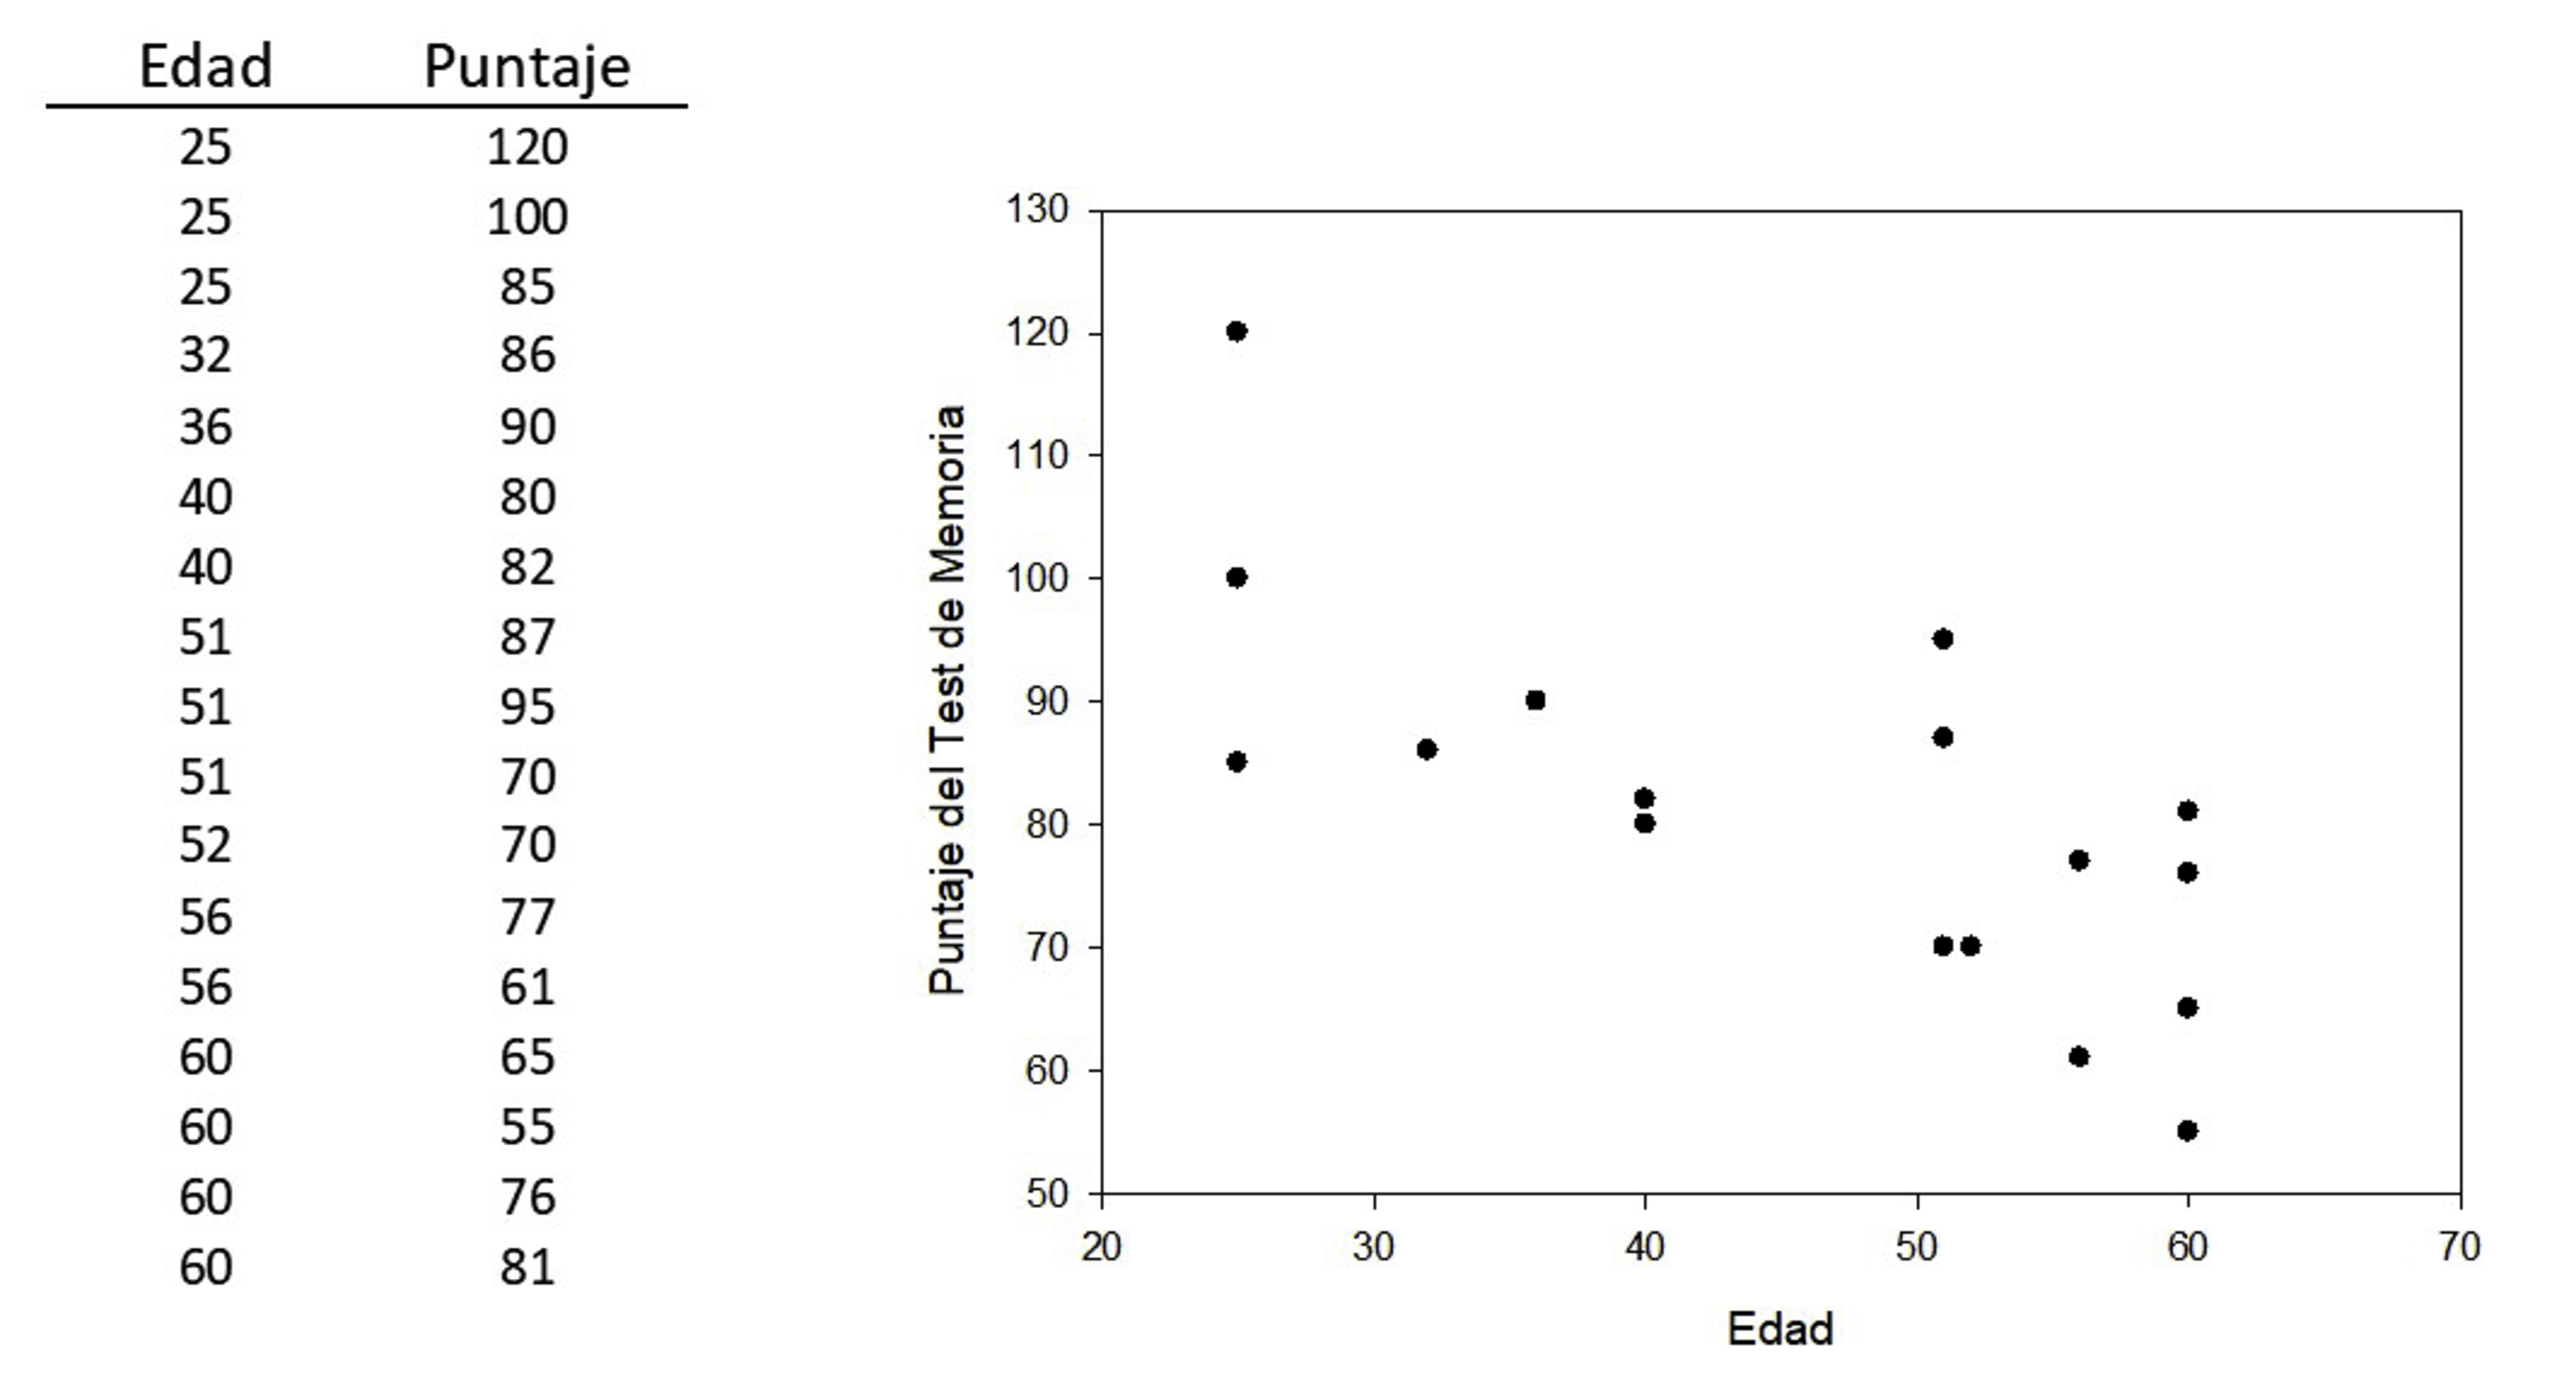
\includegraphics[width=0.9\textwidth]{tp2_fig4.jpg} 
\end{center}
\begin{enumerate} [leftmargin=2cm]
\item Hay edades para las cuales hay más de un puntaje. ¿Qué significado tiene esto? 
\item ¿Cómo está representado esto en el gráfico?
\item ¿Cómo reconocemos en un gráfico xy si la relación graficada es o no una función? 
\item  En el mismo estudio, ahora se considera para cada edad, el promedio del puntaje obtenido en todas las personas que resolvieron el test, según su edad. ¿Es esta una función? Explicar. Proponer un gráfico para esta situación.
\end{enumerate}

%13
\item Tomemos ahora el siguiente ejemplo, donde tenemos una función definida por una tabla.  En un globo aerostático se miden continuamente la temperatura del aire (en °C) y la altura sobre el nivel del mar (en msnm). Los datos de la tabla son los que corresponden a la temperatura a diferentes alturas:\\

\begin{center} 
\begin{tabular}{l c c c c c c}
\hline
x (msnm)&10 &100 &200 & 500 & 1000 &2400 \\
\hline
y (°C)	& 9,95 & 9,5 & 9 & 7,5 & 5 &-2\\
\hline
\end{tabular}
\end{center}
\begin{enumerate} [leftmargin=2cm]
\item ¿Qué información sería ésta, por ejemplo?
\item ¿Es posible deducir de esta información cuál será la temperatura a los 1500 m de altura?
\item ¿Es posible deducir de esta información a qué altura  la temperatura será de 0°C? 
\item ¿Cómo estamos seguros de que en este caso la relación mostrada en la tabla es una función?
\item Graficar esta relación.
\item Este tipo de presentación de los datos de una función es una muestra siempre parcial de la información que podemos tener. ¿Cómo sería el gráfico de la función $y = f(x)$ en este caso (la temperatura del aire en función de la altura del globo)?
\item ¿Cuál es el dominio de esta función? ¿Y cuál es la imagen?
\end{enumerate}

%14
\item Si en vez de tener una tabla de valores pudiéramos tener una fórmula que nos permitiera calcular la temperatura del aire en función de la altura del globo, tendríamos una visión completa de la variación de la variable dependiente en función de la variación de la variable independiente.\\
Supongamos que  $y=f(x)=10-\frac{1}{200}x$. Esto significa que si elegimos cualquier altura $x$, podemos calcular el valor de la temperatura $y$, reemplazando $x$ en la fórmula. Por ejemplo: \\
\begin{itemize*} [leftmargin=2cm]
\item Si $x = 20$ metros, $y=f(20)=10- \frac{1}{200}20=9.9\,^\circ \text{C}$ \\
\item Si $x = 4000$ metros, $y=f(4000)=10- \frac{1}{200}4000=-10 \,^\circ \text{C}$
\end{itemize*}

La información dada por esta fórmula  es mucho más completa. Por ejemplo pueden contestarse diferentes preguntas (contestarlas):
\begin{enumerate} [leftmargin=2cm]
\item ¿Cuál es la temperatura del aire justo al nivel del mar?
\item ¿A qué altura sobre el nivel del mar la temperatura comienza a ser inferior a los 0°C?
\item ¿Cuál es la temperatura a los 300 msnm?
\item ¿A qué altura la temperatura es de 7 °C? 
\end{enumerate}

También esta forma de representación de la función mediante una fórmula puede trasladarse a un gráfico.

\begin{enumerate} [leftmargin=2cm,resume*]
\item Realizar el gráfico (podés usar el graficador).
\item Ubicar en el gráfico anterior los puntos de la tabla de información inicial.
\item El gráfico de la función es una recta. ¿Había alguna posibilidad de saber esto desde el análisis de los datos de la tabla?
\item El análisis del gráfico anterior nos permite decir que la temperatura decrece con la altura. ¿Podíamos decir eso desde la tabla? 
\end{enumerate}

%15
\item Supongamos que tenemos la función $f(x)=x^2-2x+1$.
\begin{enumerate}
\item Calcular $f(2)$, $f(0)$ y $f(-1)$.
\item ¿Cómo hacemos para saber si el punto $(1,0)$ y el punto $(3,2)$ pertenecen a la gráfica de la función?. Verificarlo.
\end{enumerate}

%16
\item  En un estudio sobre las condiciones de reproducción de cierta colonia de bacterias se observó la influencia de la temperatura sobre el número de las mismas. El gráfico obtenido se muestra a continuación. Se pide contestar:
\begin{enumerate} [leftmargin=2cm]
\item ¿Cuál es la variable dependiente y cuál la variable independiente?
\item En el eje vertical cada segmento representa 10000 bacterias. ¿Cuánto representa cada segmento del eje horizontal?
\item ¿Cuántas bacterias se encontraron a los 10 °C de temperatura?
\item ¿A qué temperatura se llega al mayor número de bacterias? 
\item ¿Cuál será la temperatura adecuada para combatir a esa bacteria?
\end{enumerate}
\begin{center} 
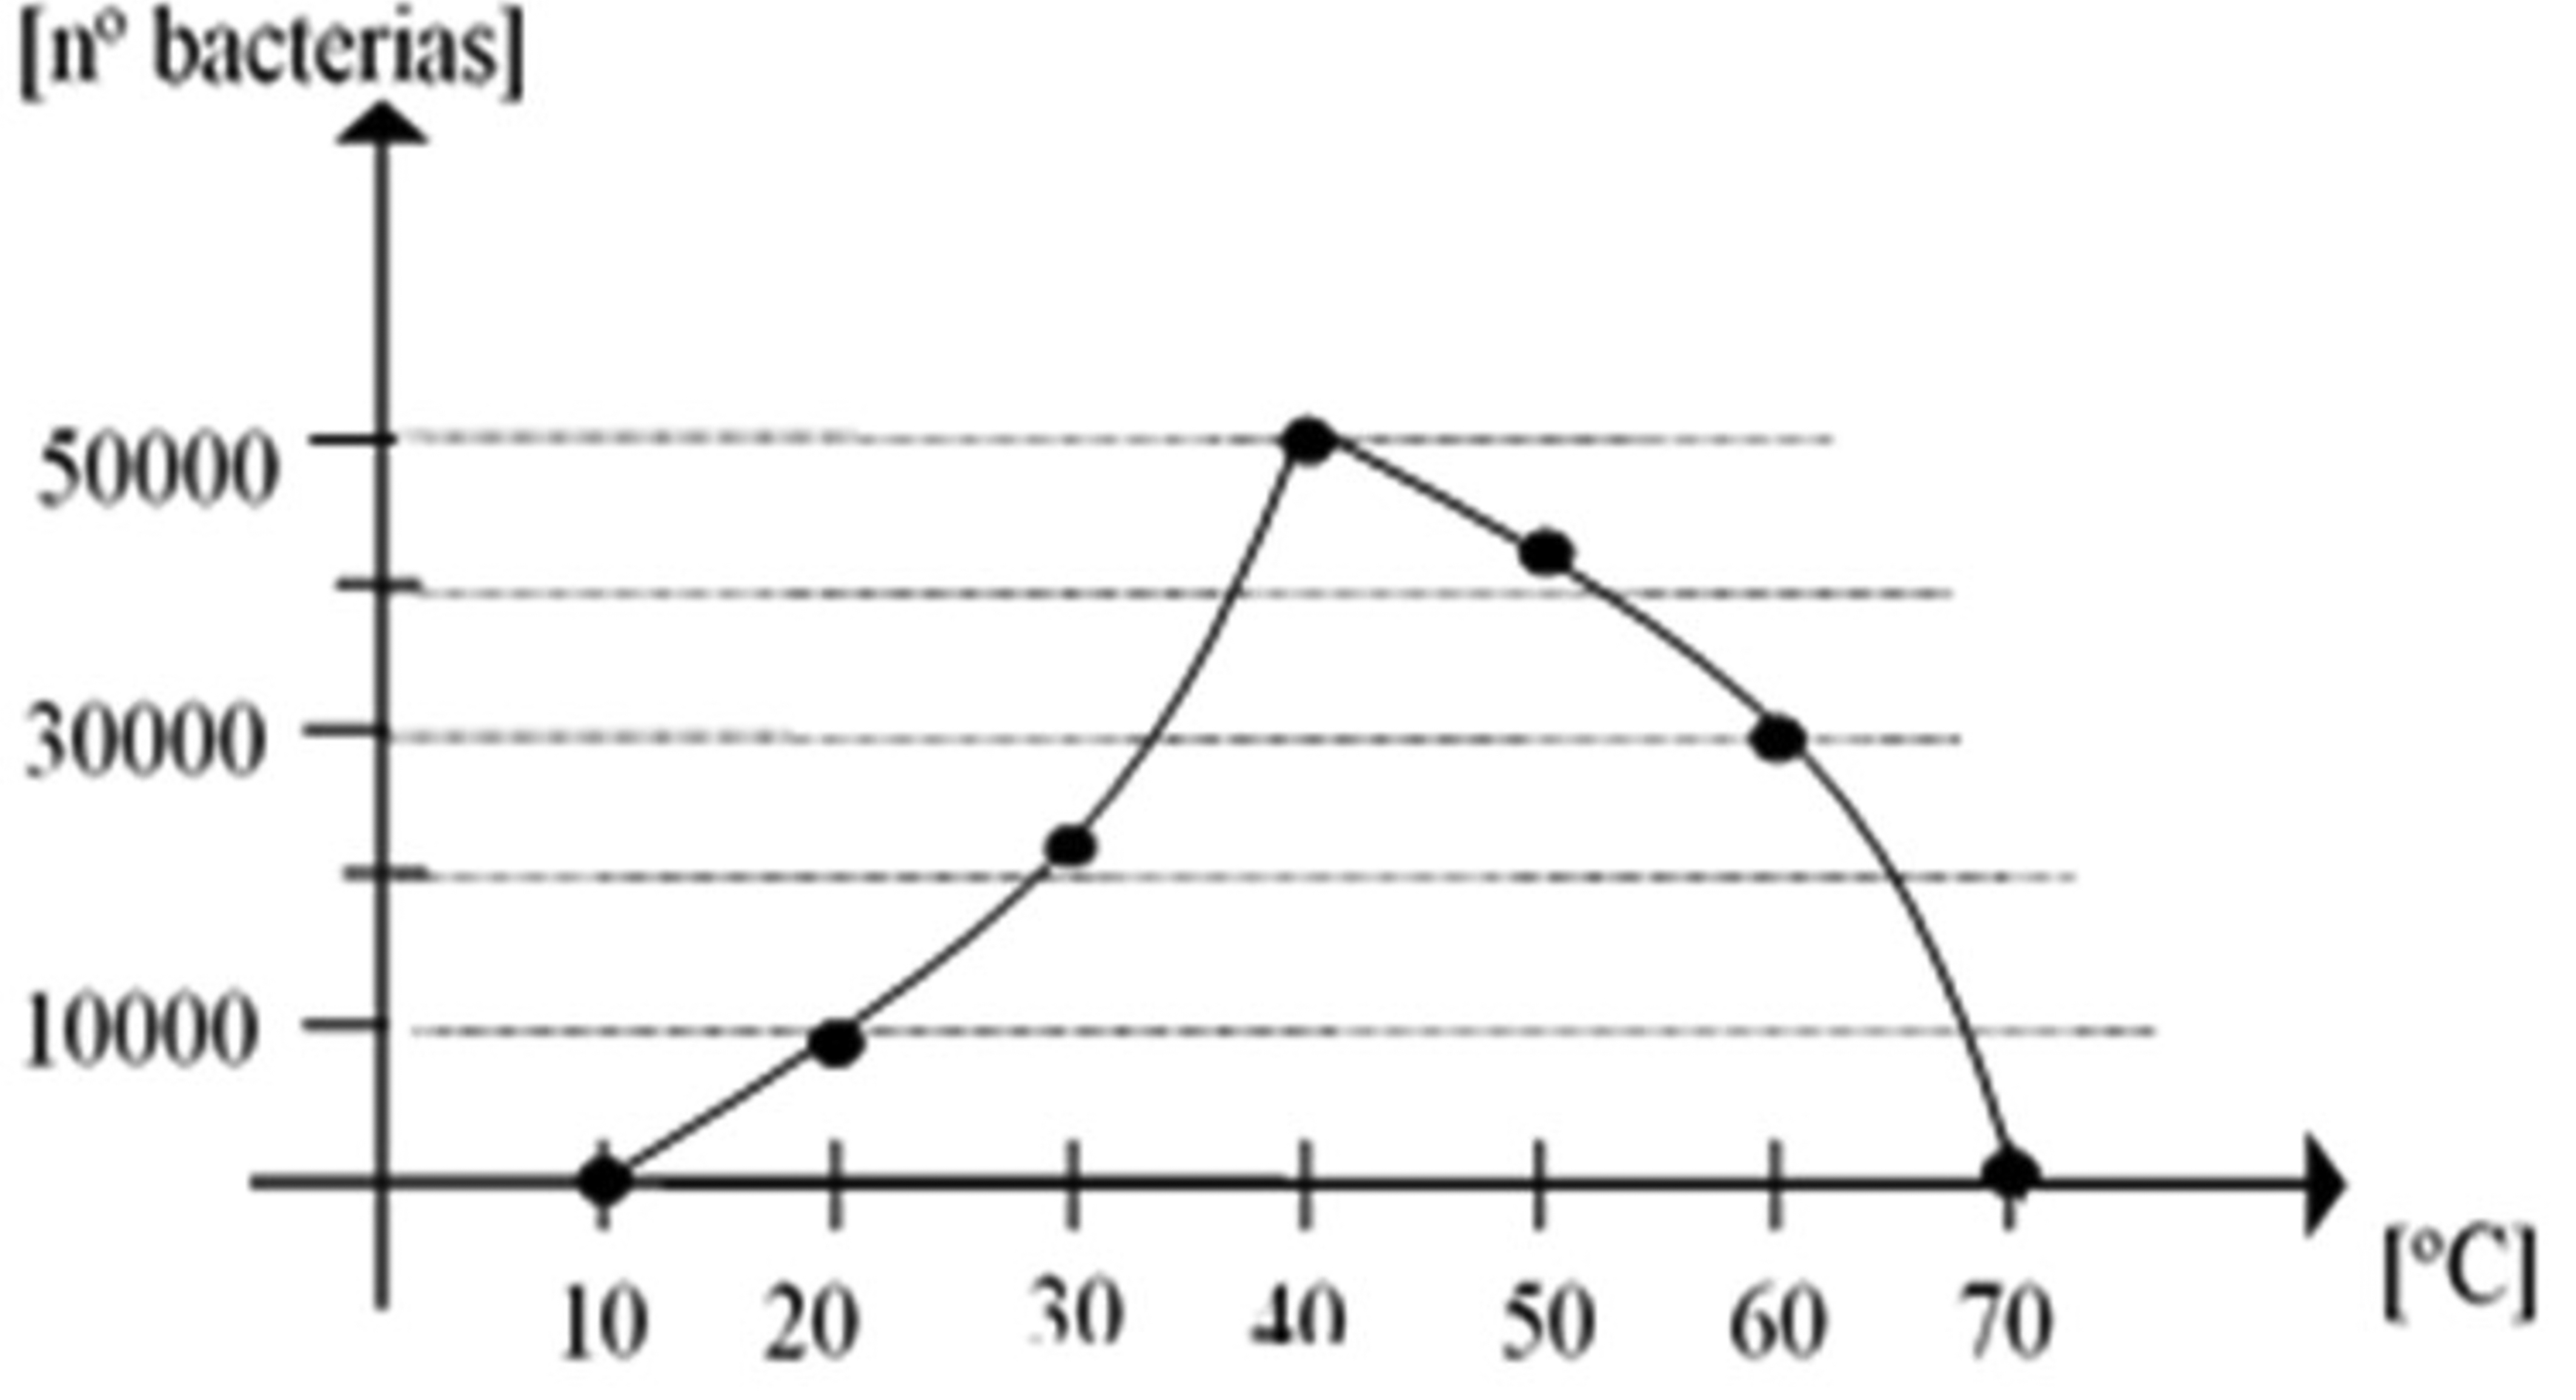
\includegraphics[width=0.5\textwidth]{tp2_fig6.jpg} 
\end{center}

%17
\item  Inventar un gráfico que podría estar mostrando la siguiente información:
\begin{enumerate} [leftmargin=2cm]
\item La cantidad promedio de agua consumida mensualmente (en litros) de acuerdo a la cantidad de habitantes del domicilio en el que se encuentra colocado el medidor.
\item El costo de una llamada telefónica desde un teléfono público en función del tiempo que dura la llamada, con las siguientes condiciones: los primeros dos minutos cuestan 56 centavos, luego, cada dos minutos se cobran 23 centavos adicionales.
\item La cantidad de energía eléctrica que se consume en una casa durante las 24 horas de un día (pensar que siempre hay algo prendido,  como la heladera). 
\end{enumerate}

%18
\item En el inciso (a) del punto anterior tenemos un ejemplo del gráfico de una relación entre una variable dependiente continua y una variable independiente discreta (en este caso el dominio de la función es un subconjunto de los números naturales). En el inciso (c) tenemos el caso de un gráfico que relaciona dos variables continuas. En el (b), en cambio, la variable dependiente es discreta y la variable independiente continua. Proponer ejemplos de gráficos que relacionen dos variables discretas y ejemplos de gráficos que relacionen una variable dependiente discreta y una variable independiente continua o al revés. Discutir las diferencias que estas relaciones muestran en los gráficos.

\fbox{ \parbox{0.98\linewidth}{
\noindent
\textbf{Precisamos los conceptos.}\\
\begin{itemize*} [leftmargin=2cm]
\item Para designar una función que tiene dominio en $A$ y conjunto de llegada (o codominio) $B$ se utiliza la siguiente notación $f: A  \rightarrow  B$, y se lee “ \textit{f va de A en B}”.\\
\item En general simbolizaremos con $x$ a los elementos del dominio y con $y$ a los elementos del codominio.\\
\item El dominio de una función $f$ es el conjunto de valores que puede tomar $x$,\\
\item Cada elemento de $y$ que está asociado a une elemento de $x$ se denomina \textbf{imagen de x}, y se simboliza $y = f(x)$, y se lee: “la imagen de x por la función f es y”. A $x$ se lo denomina  \textbf{preimagen de y}.\\
\item El conjunto formado por todas las imágenes de los elementos del dominio de $f$ se llama \textbf{conjunto imagen} de f (también rango), o simplemente “imagen de f” y se simboliza $Im(f)$.\\
\item El conjunto imagen de $f$ está incluido en el codominio de $f$.\\
\item  Gráficamente:\\
\end{itemize*}
\begin{center} 
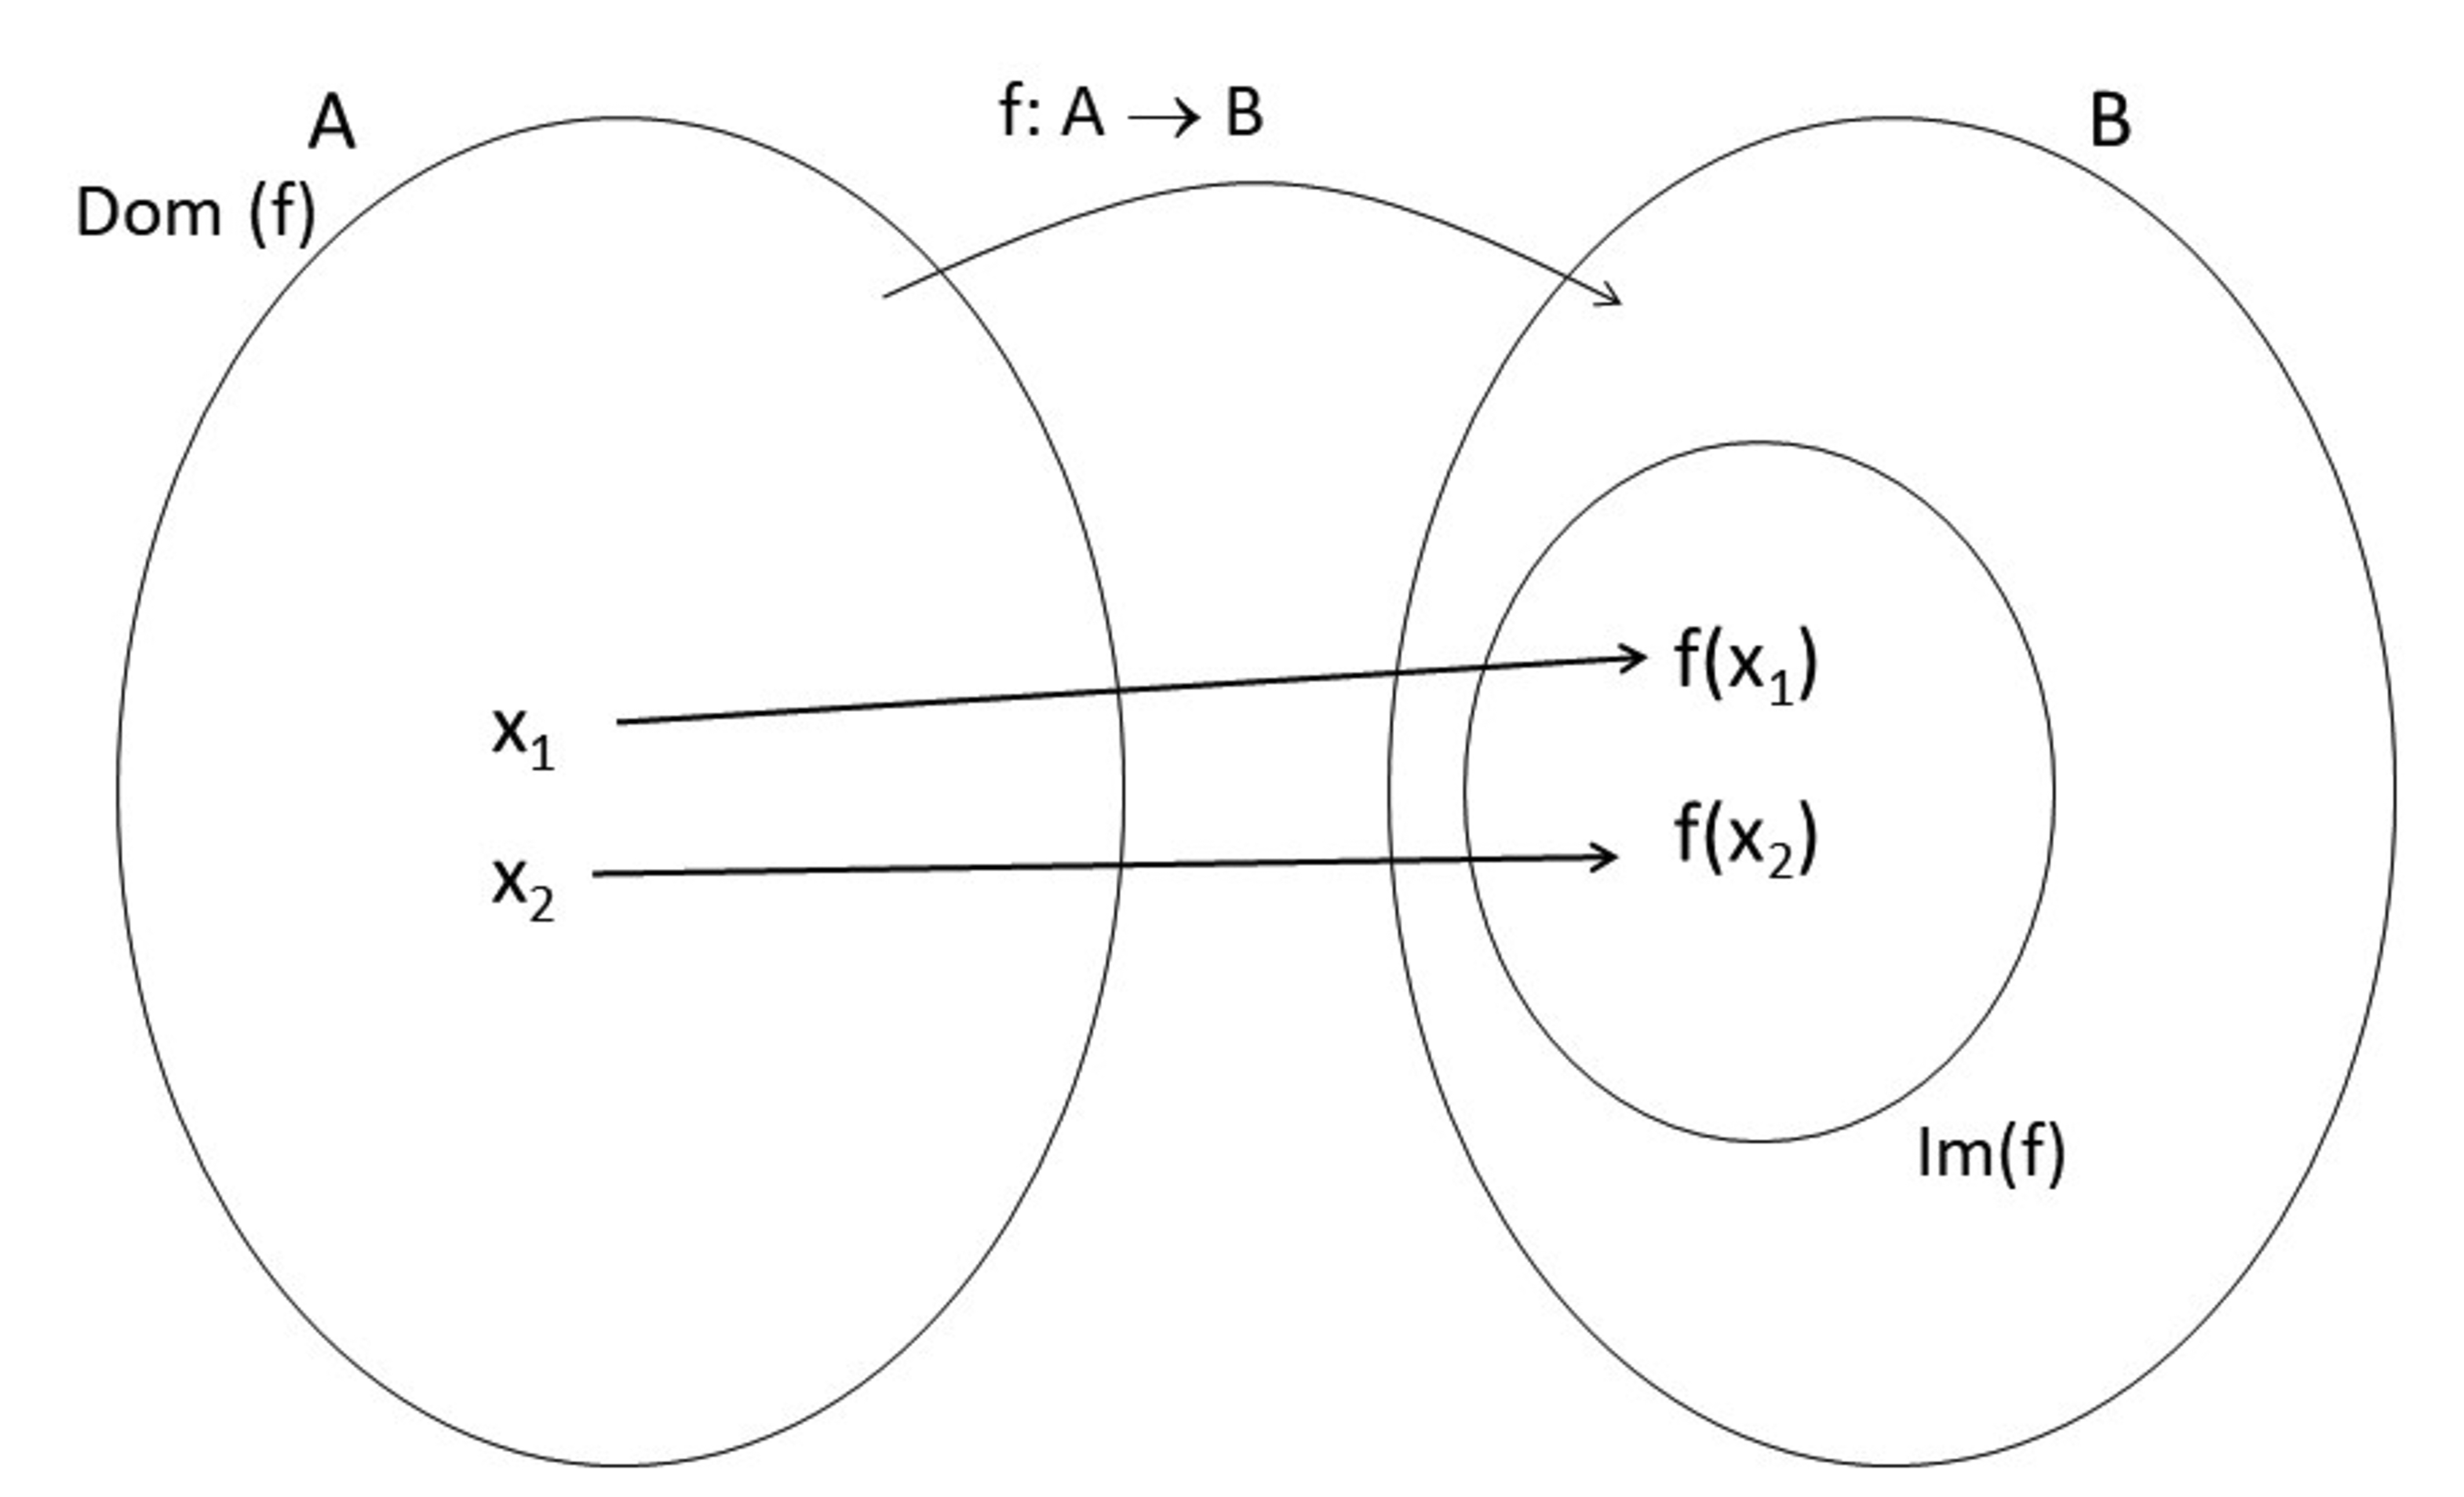
\includegraphics[width=0.6\textwidth]{tp2_fig7.jpg} 
\end{center}
}}

\vspace{0.5 cm}

\fbox{ \parbox{0.98\linewidth}{
\noindent
\textbf{Ceros, conjunto de positividad, conjunto de negatividad.}\\
\begin{mydef}  \textbf{Ceros de una función.}\\
\noindent
Llamamos  \textbf{ceros} de una función o  \textbf{raíces}, a los puntos donde la función toma el valor $0$, es decir, son los elementos del dominio de la función tales que $f(x) = 0$. Gráficamente, los ceros son los puntos del dominio donde la función corta al eje horizontal. \\
\end{mydef}
\begin{mydef}  \textbf{Conjuntos de positividad y negatividad de una función.}\\
\noindent
\begin{itemize*} [leftmargin=2cm]
\item Llamaremos \textbf{conjunto de positividad} de una función $f$ al el subconjunto del dominio para el cual las imágenes son números positivos, es decir, conjunto:
\end{itemize*}
\begin{equation*}
C^+ = \{x \in Dom(f) / f(x) > 0 \}
\end{equation*}
Gráficamente,el conjunto de positividad está representado por la unión de todos los subconjuntos del dominio (en el eje de horizontal) donde la curva que representa la función se encuentra por encima del mismo.\\
\begin{itemize*} [leftmargin=2cm]
\item Llamaremos \textbf{conjunto de negatividad} de una función $f$ al el subconjunto del dominio para el cual las imágenes son números negativos, es decir, conjunto:
\end{itemize*}
\begin{equation*}
C^- = \{x \in Dom(f)/ f(x) < 0 \}
\end{equation*}
Gráficamente,el conjunto de negatividad está representado por la unión de todos los subconjuntos del dominio (en el eje de horizontal) donde la curva que representa la función se encuentra por debajo del mismo.
\end{mydef}
Consideremos la función del siguiente gráfico, con dominio en todos los reales, es decir, $f:  \mathbb{R} \rightarrow  \mathbb{R}$. En el gráfico de la izquierda marcamos el conjunto de positividad, y en el de la derecha, el conjunto de negatividad. Los puntos $x_0$, $x_1$ y $x_2$ son los ceros de la función. \\

\begin{center} 
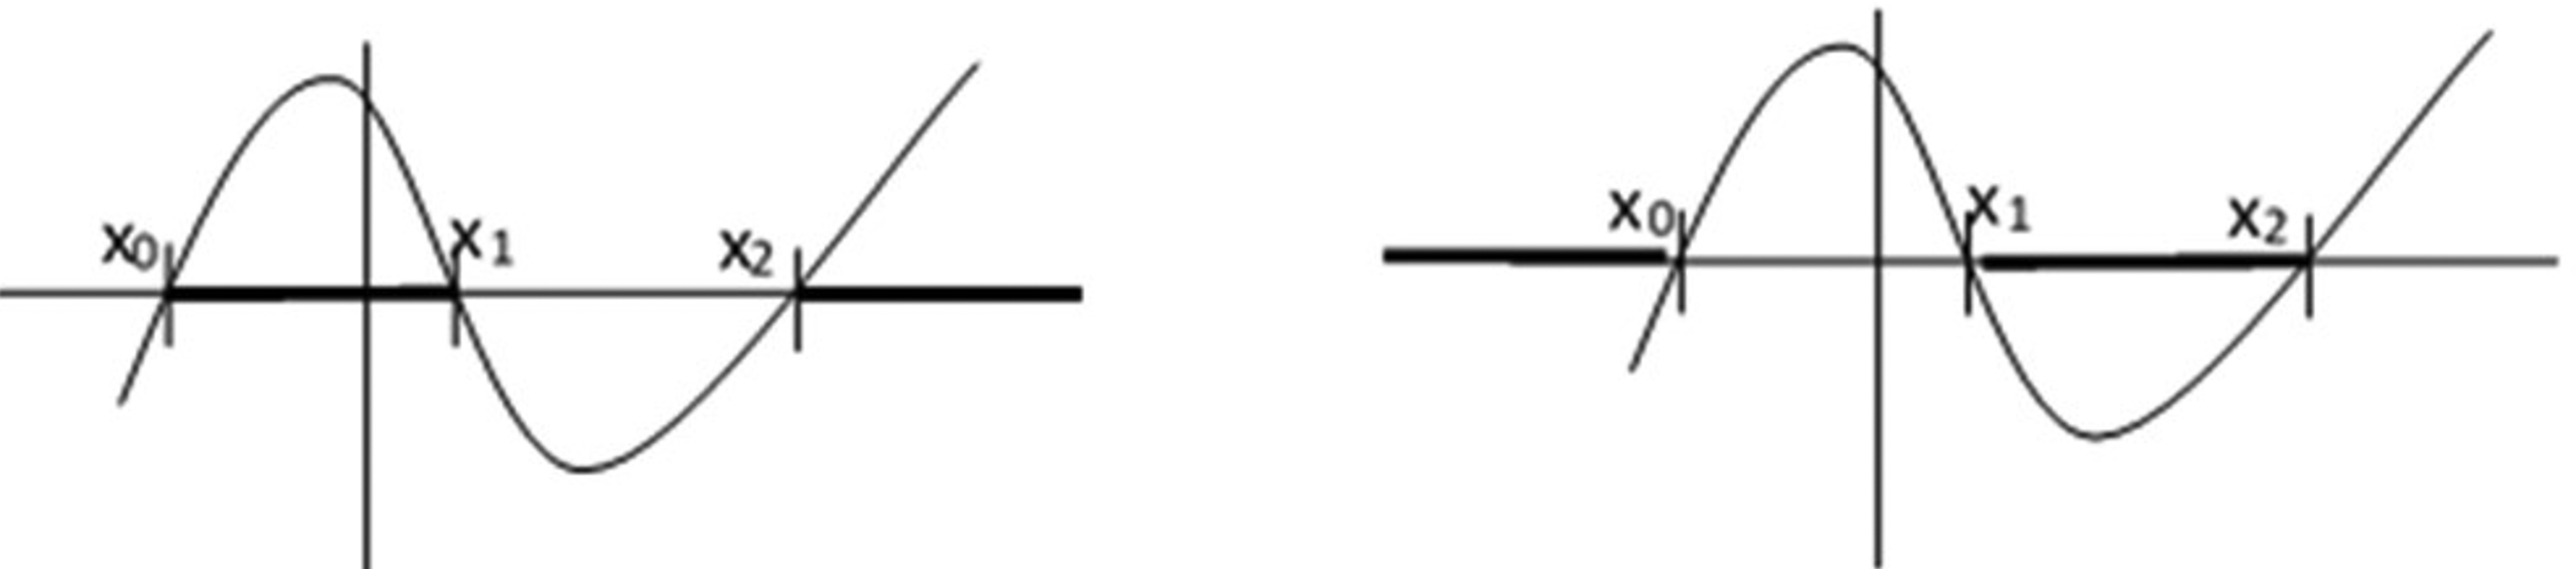
\includegraphics[width=0.8\textwidth]{tp2_fig9.jpg} 
\end{center}
\begin{equation*}
C^+ = (x_0, x_1) \cup (x_2,+\infty) \text{      y     }  C^- = (-\infty,x_0) \cup (x_1,x_2)
\end{equation*}

}}
\vspace{0.8 cm}


%19
\item Determinar los ceros de las siguientes funciones:
\begin{center} 
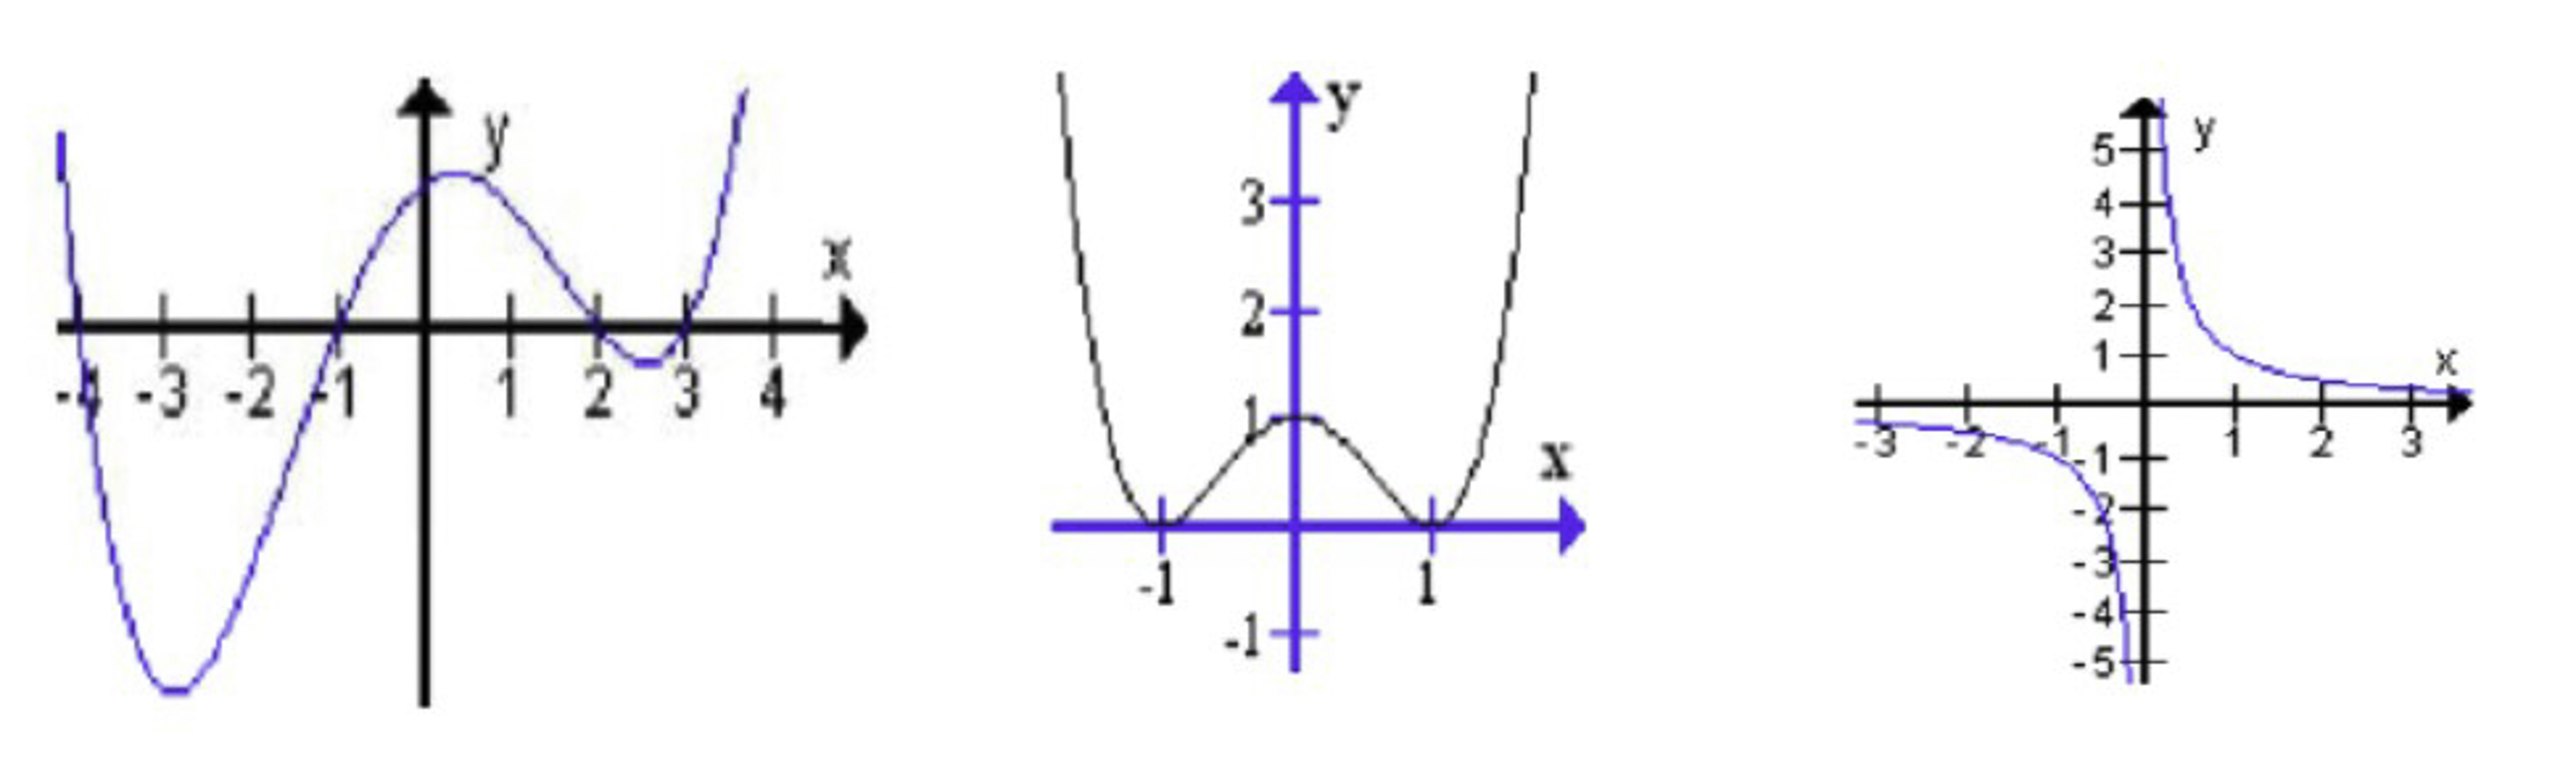
\includegraphics[width=0.6\textwidth]{tp2_fig8.jpg} 
\end{center}

%20
\item Una función puede tener desde ningún cero hasta infinitos ceros. Inventar gráficos de funciones que tengan a) ningún cero, b) un cero,  c) dos ceros,   d) tres ceros,   e) infinitos ceros.

%21
\item La determinación analítica de los ceros de una función es en ocasiones difícil (si no imposible), dependiendo del grado de complejidad de la función analizada. Sin embargo cuando la función es sencilla, el cálculo analítico se traduce a la resolución de ecuaciones simples. Encontrar los ceros de las siguientes funciones:\\
\begin{multicols}{2}
\begin{enumerate} [leftmargin=2cm]
\item $f(x) = 2x - 3$ 
\item  $f(x) =  x^2-x$
\item $f(x) = \frac{12}{x}-3$ 
\item  $f(x) = \frac{x+2}{x^2+1}$
\end{enumerate}
\end{multicols}

\vspace{0.3 cm}
%22
\item En los siguientes gráficos indicar dominio e imagen. Marcar en el eje de las x los ceros, conjuntos de positividad y de negatividad. Escribir estos conjuntos.
\begin{center} 
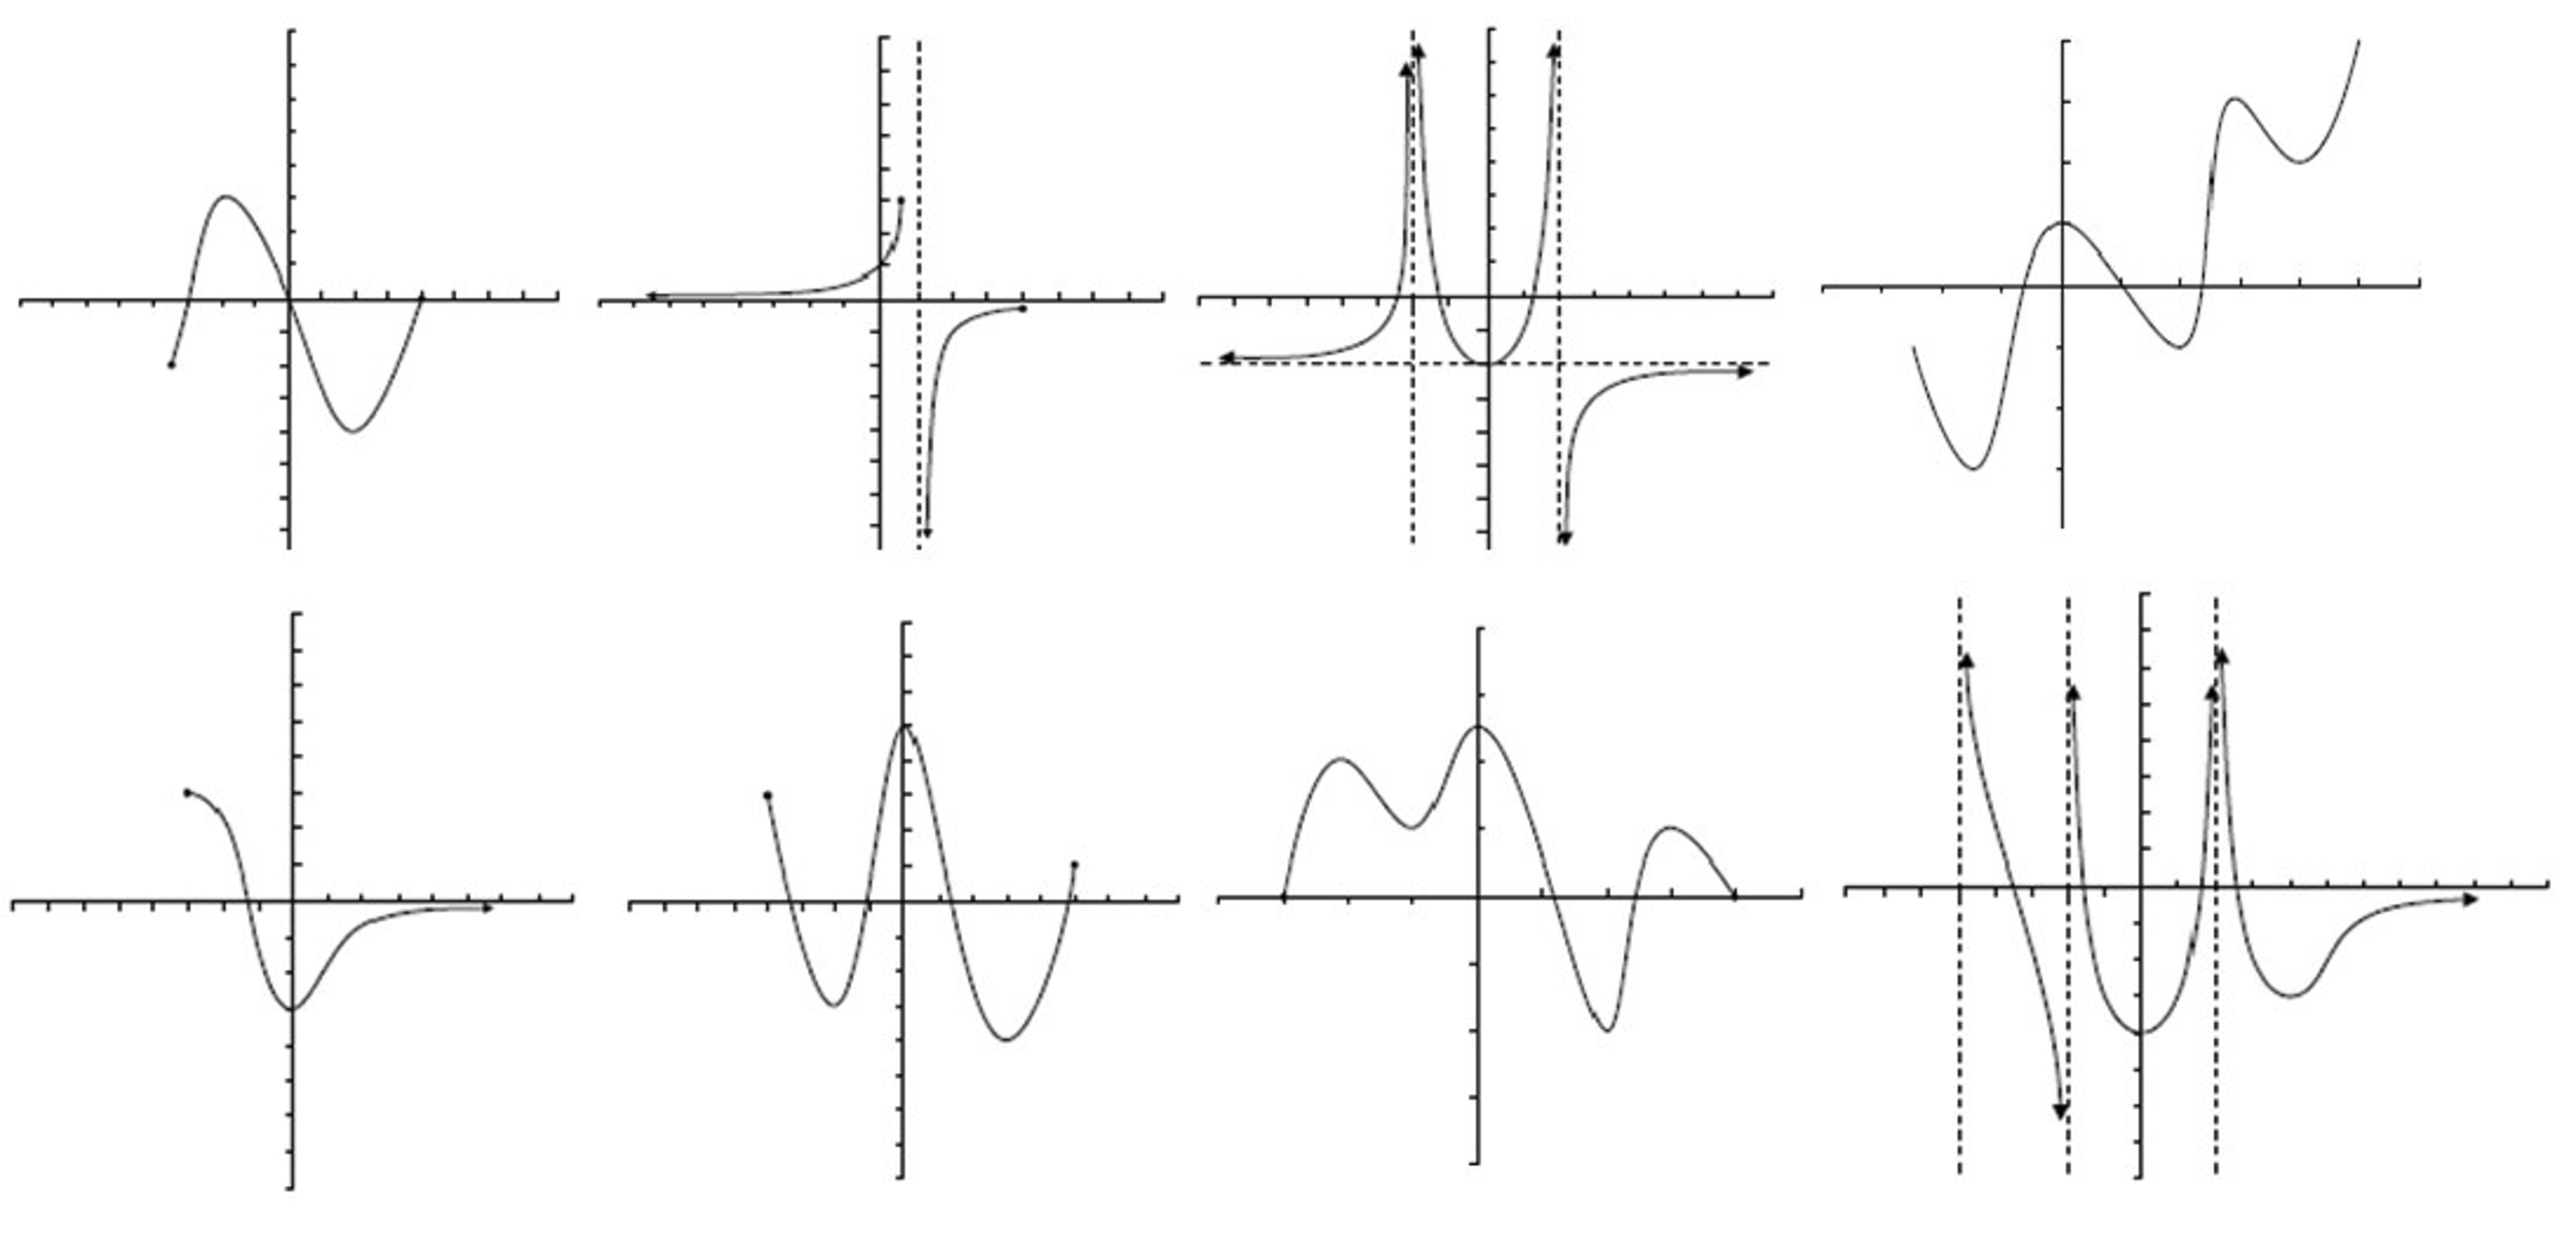
\includegraphics[width=0.98\textwidth]{tp2_fig11.jpg} 
\end{center}

\fbox{ \parbox{0.98\linewidth}{
\noindent
\begin{mydef}  \textbf{Intervalos de crecimiento y decrecimiento.}\\
Una función \textbf{crece} en un intervalo si siempre que se toman dos puntos de ese intervalo, la imagen del menor es más chica que la imagen del mayor. Es decir: si para todo par de valores dentro de un intervalo tales que  $x_1 < x_2$ tenemos que   $f(x_1) < f(x_2)$ diremos que la función  \textbf{crece} en el intervalo.\\
Una función \textbf{decrece} en un intervalo si siempre que se toman dos puntos de ese intervalo, la imagen del menor es más grande que la imagen del mayor. Es decir: Si para todo par de valores dentro de un intervalo tales que $x_1 < x_2$ tenemos que   $f(x_1) > f(x_2)$ diremos que la función  \textbf{decrece} en el intervalo.\\
Es decir que una función decrece en un intervalo si siempre que se toman dos puntos de ese intervalo, la imagen del menor, es más grande que la imagen del mayor. \\
Gráficamente: 
\begin{center} 
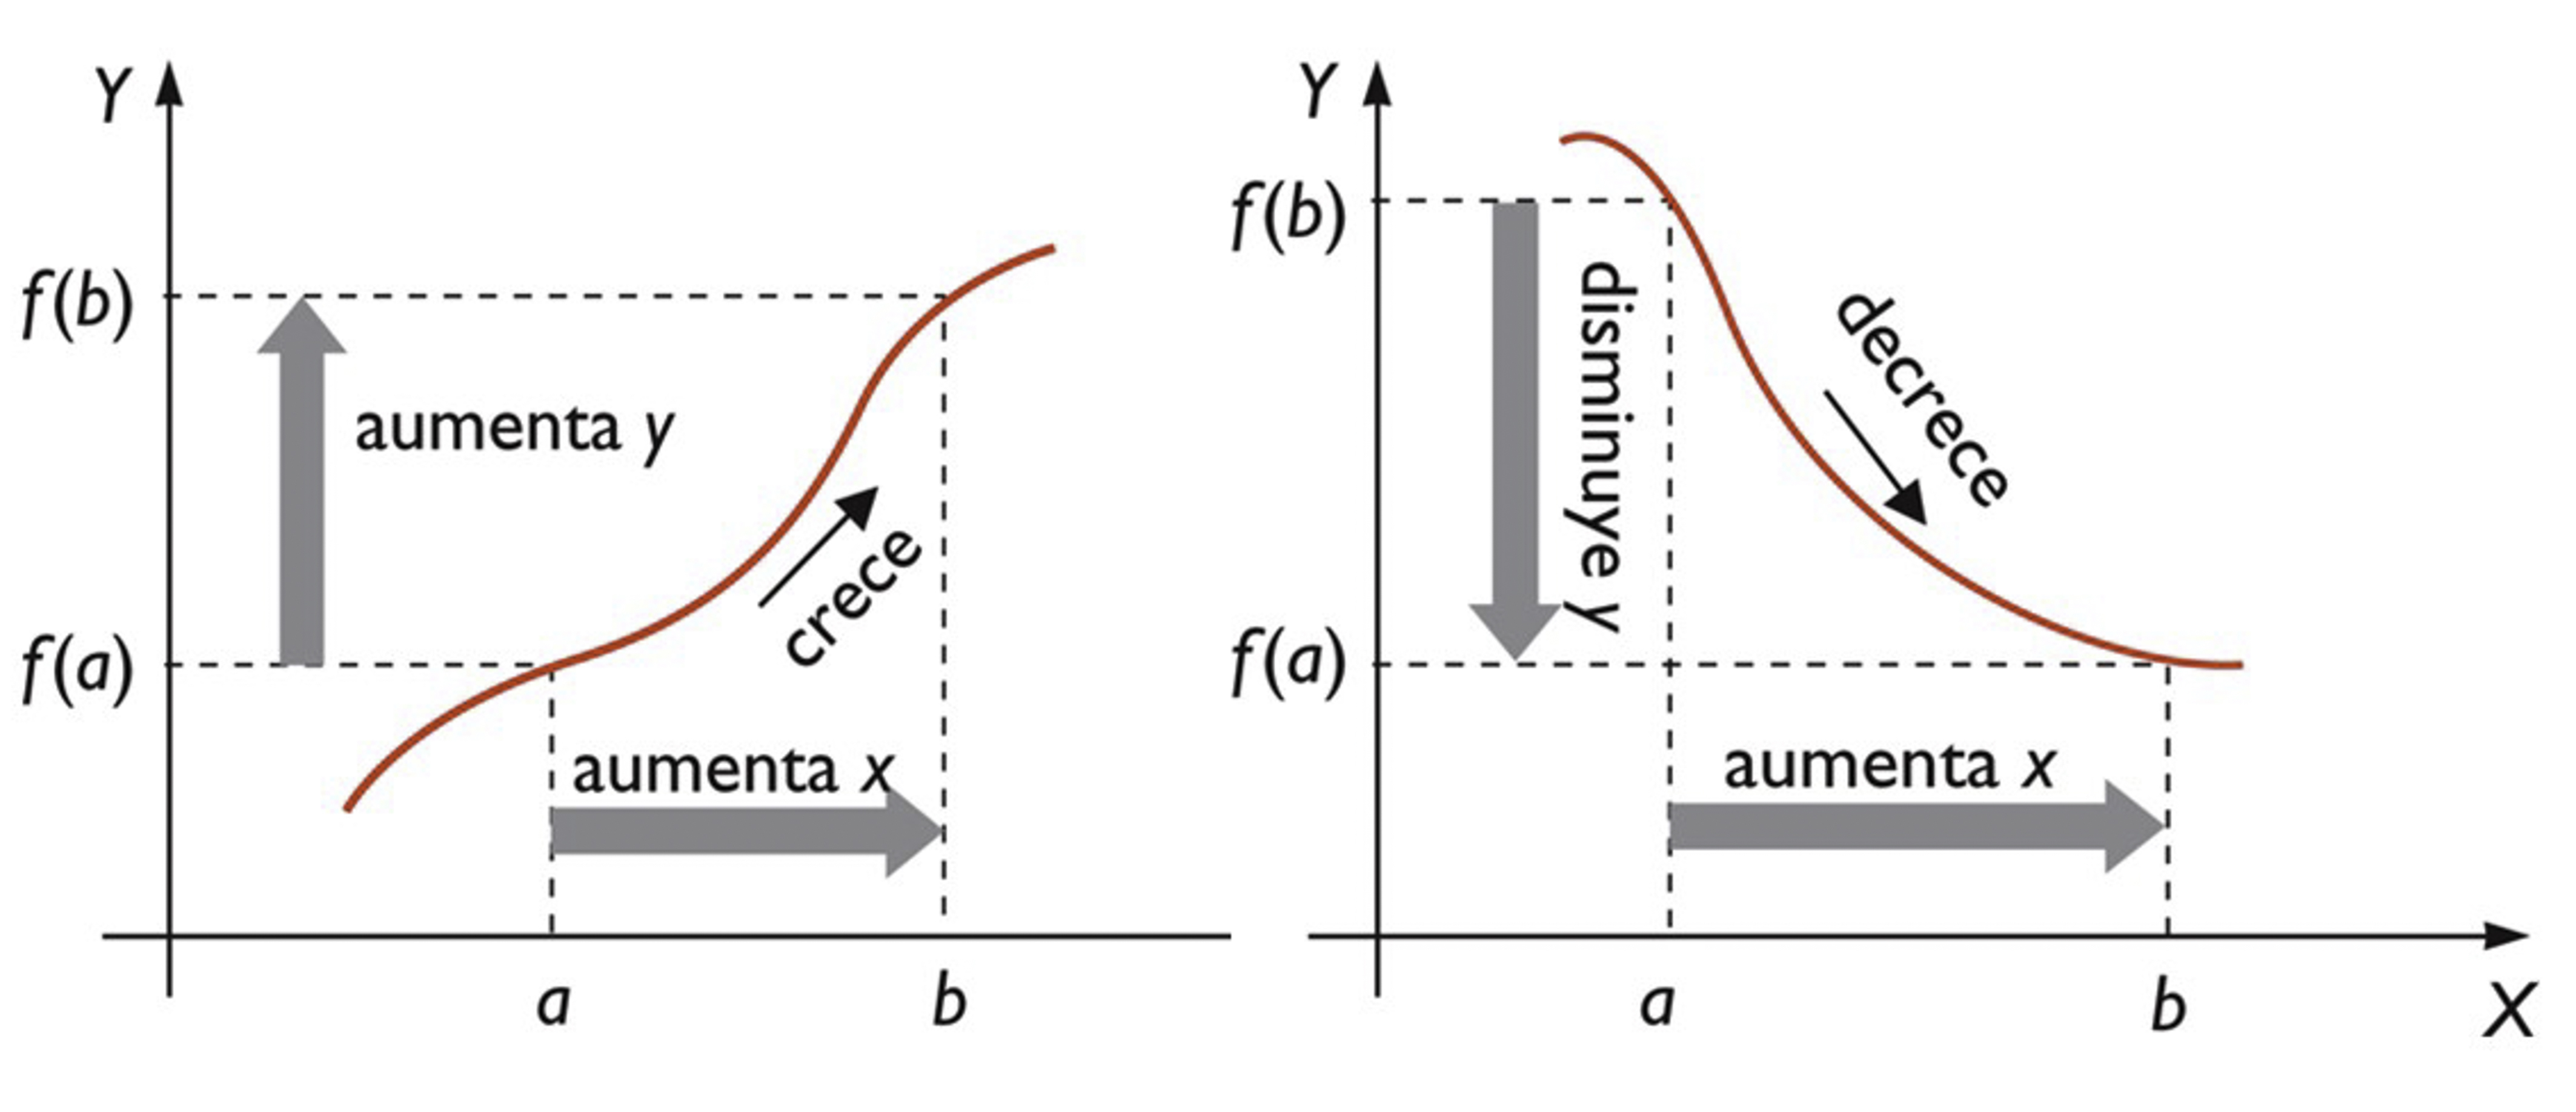
\includegraphics[width=0.98\textwidth]{tp2_fig12.jpg} 
\end{center}
\end{mydef}
}}

%24
\item En los siguientes gráficos marcar en el eje de las x intervalos de crecimiento y decrecimiento, y escribirlos lo más formalmente posible.
\begin{center} 
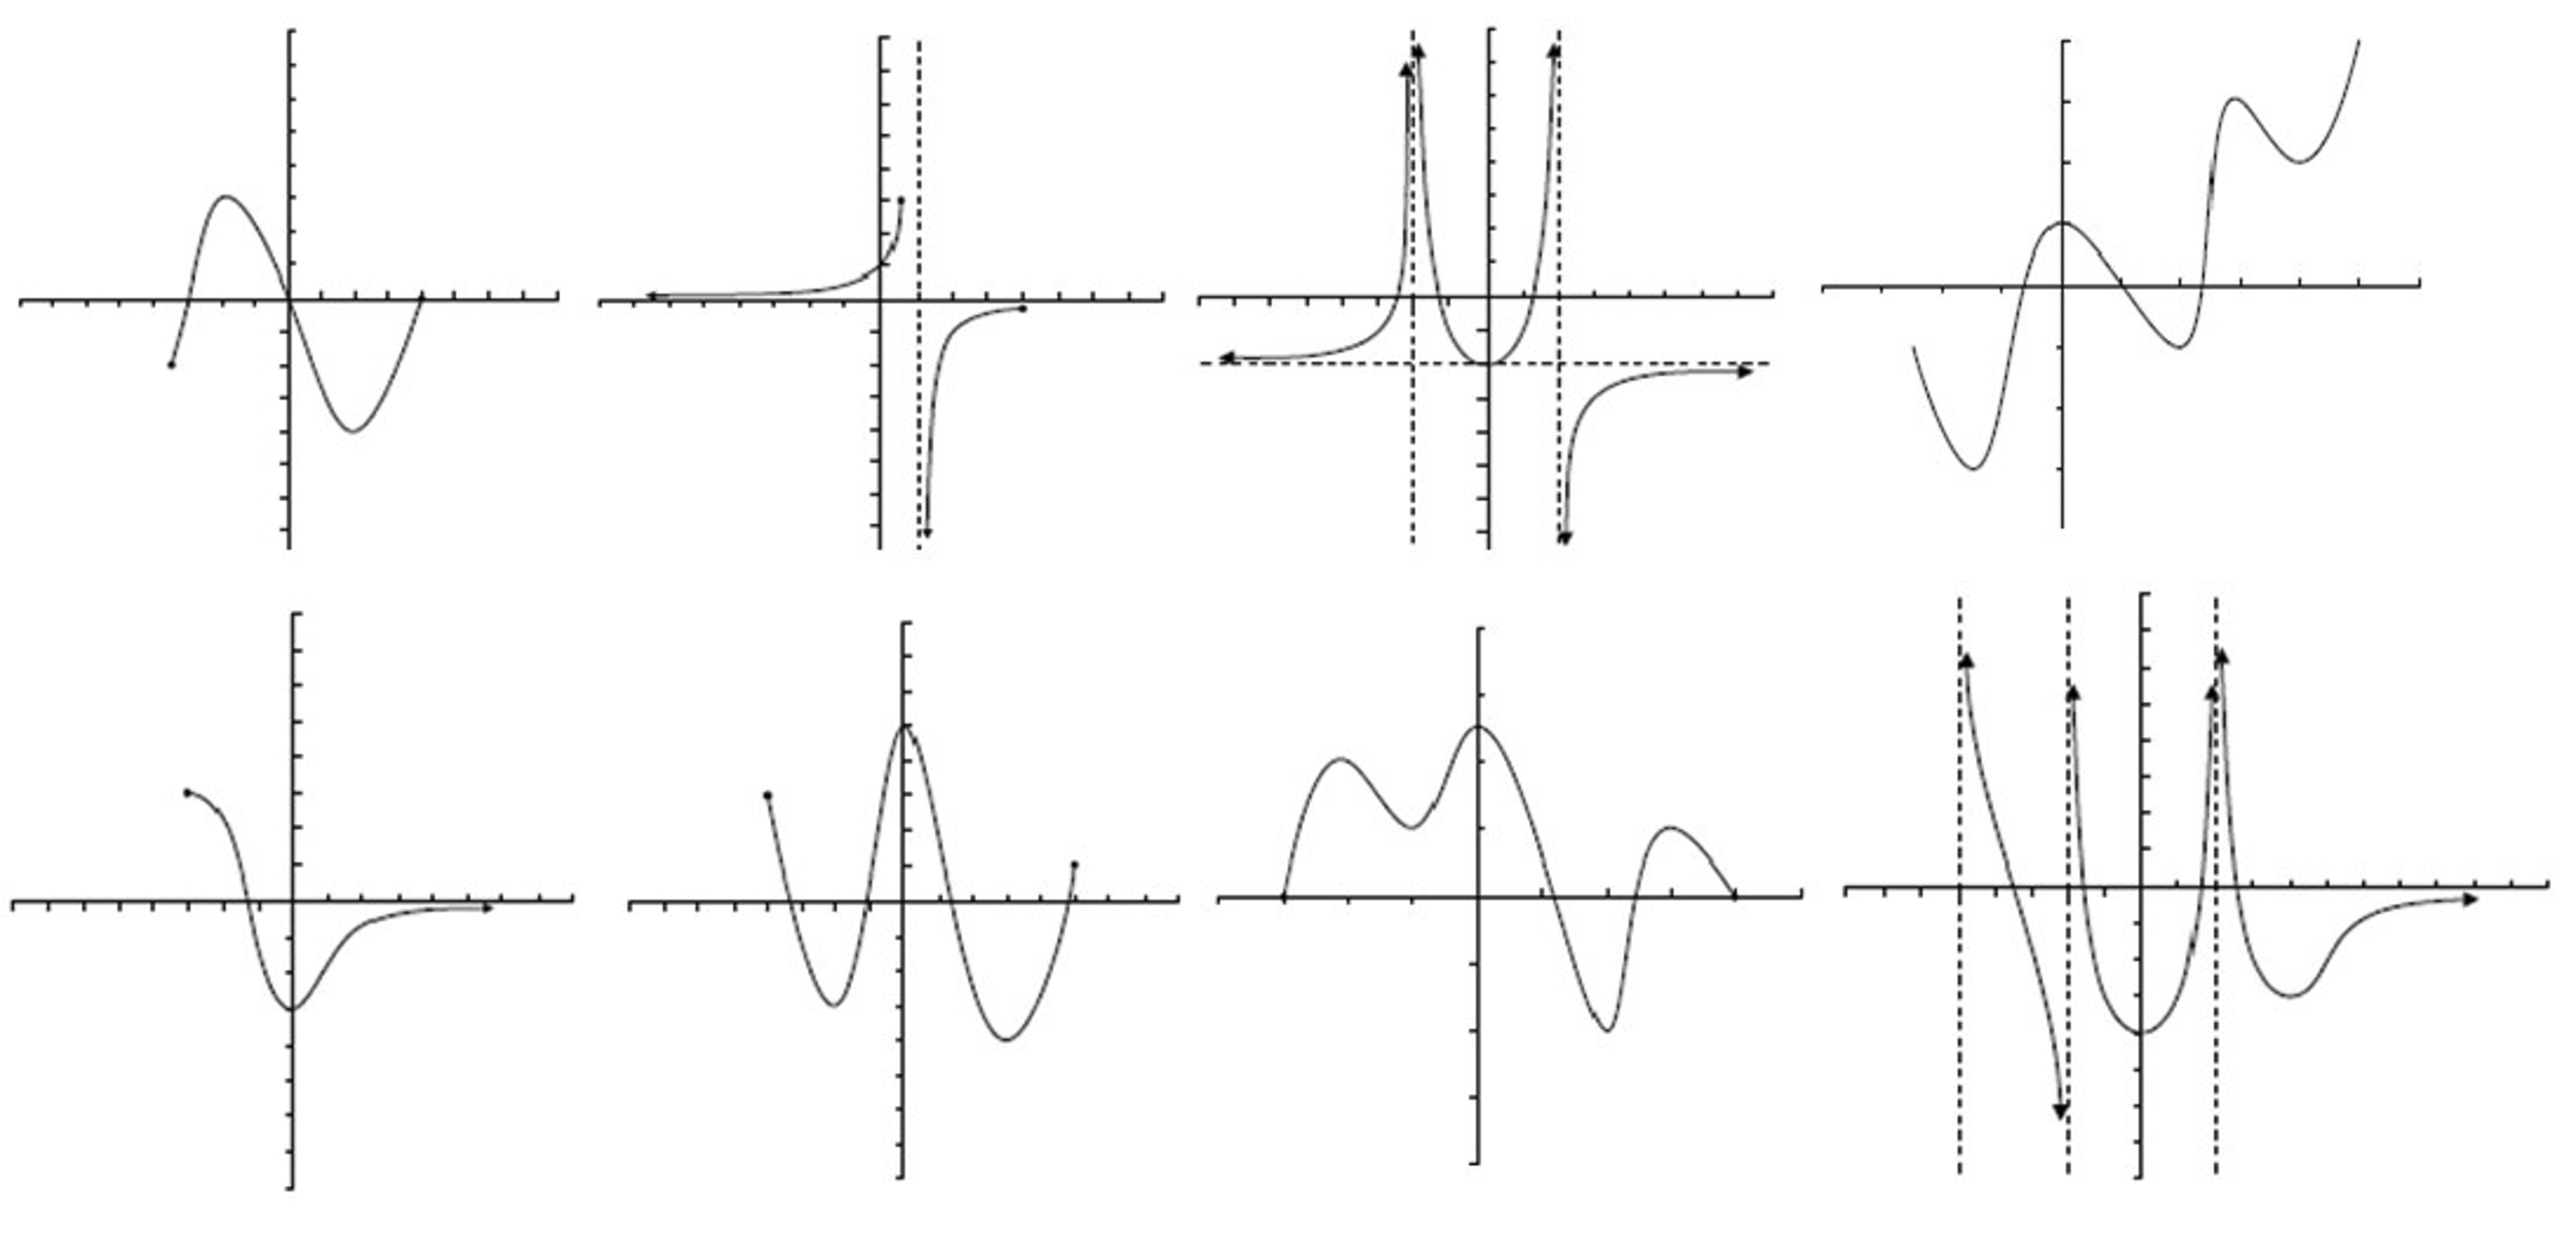
\includegraphics[width=0.98\textwidth]{tp2_fig11.jpg} 
\end{center}

\fbox{ \parbox{0.98\linewidth}{
\noindent
\textbf{Máximos y mínimos de una función.}\\
\noindent
\begin{mydef}  \textbf{Extremos locales o relativos}\\
Se dice que la función $f(x)$ alcanza un \textbf {máximo local} o relativo en $x = c$ si y solo si $f(c) \geq  f(x)$ para todo $x$ suficientemente próximo a $x = c$.\\
Se dice que la función $f(x)$ alcanza un \textbf {mínimo local} o relativo en $x = c$ si y solo si $f(c) \leq  f(x)$ para todo $x$ suficientemente próximo a $x = c$.\\
\end{mydef}
\begin{mydef}  \textbf{Extremos absolutos.}\\
Se dice que la función $f(x)$ alcanza un \textbf {máximo absoluto} en $x = d$ si y solo si $f(d) \geq  f(x)$ para todo $x$ del dominio de la función.\\
Se dice que la función $f(x)$ alcanza un \textbf {mínimo absoluto} en $x = d$ si y solo si $f(d) \leq  f(x)$ para todo $x$ del dominio de la función.\\
\end{mydef}
}}


%25
\item Mostrar ejemplos gráficos de funciones que tengan máximos y mínimos locales.

%26
\item Proponer ejemplos gráficos de funciones tales que:\\
\begin{enumerate} [leftmargin=2cm]
\item Tengan extremos absolutos.
\item Tengan extremos locales pero no absolutos.
\item Tengan extremos locales que no coincidan con los extremos absolutos.
\item ¿Es posible que una función tenga extremos que sean absolutos pero no locales? Explicar.
\item  No tenga extremos de ningún tipo.
\item  No tenga máximo ni mínimo, pero $f(-1) > f(1)$.
\end{enumerate}


%33
\item Para los siguientes gráficos determinar los máximos y mínimos locales y absolutos.
\begin{center} 
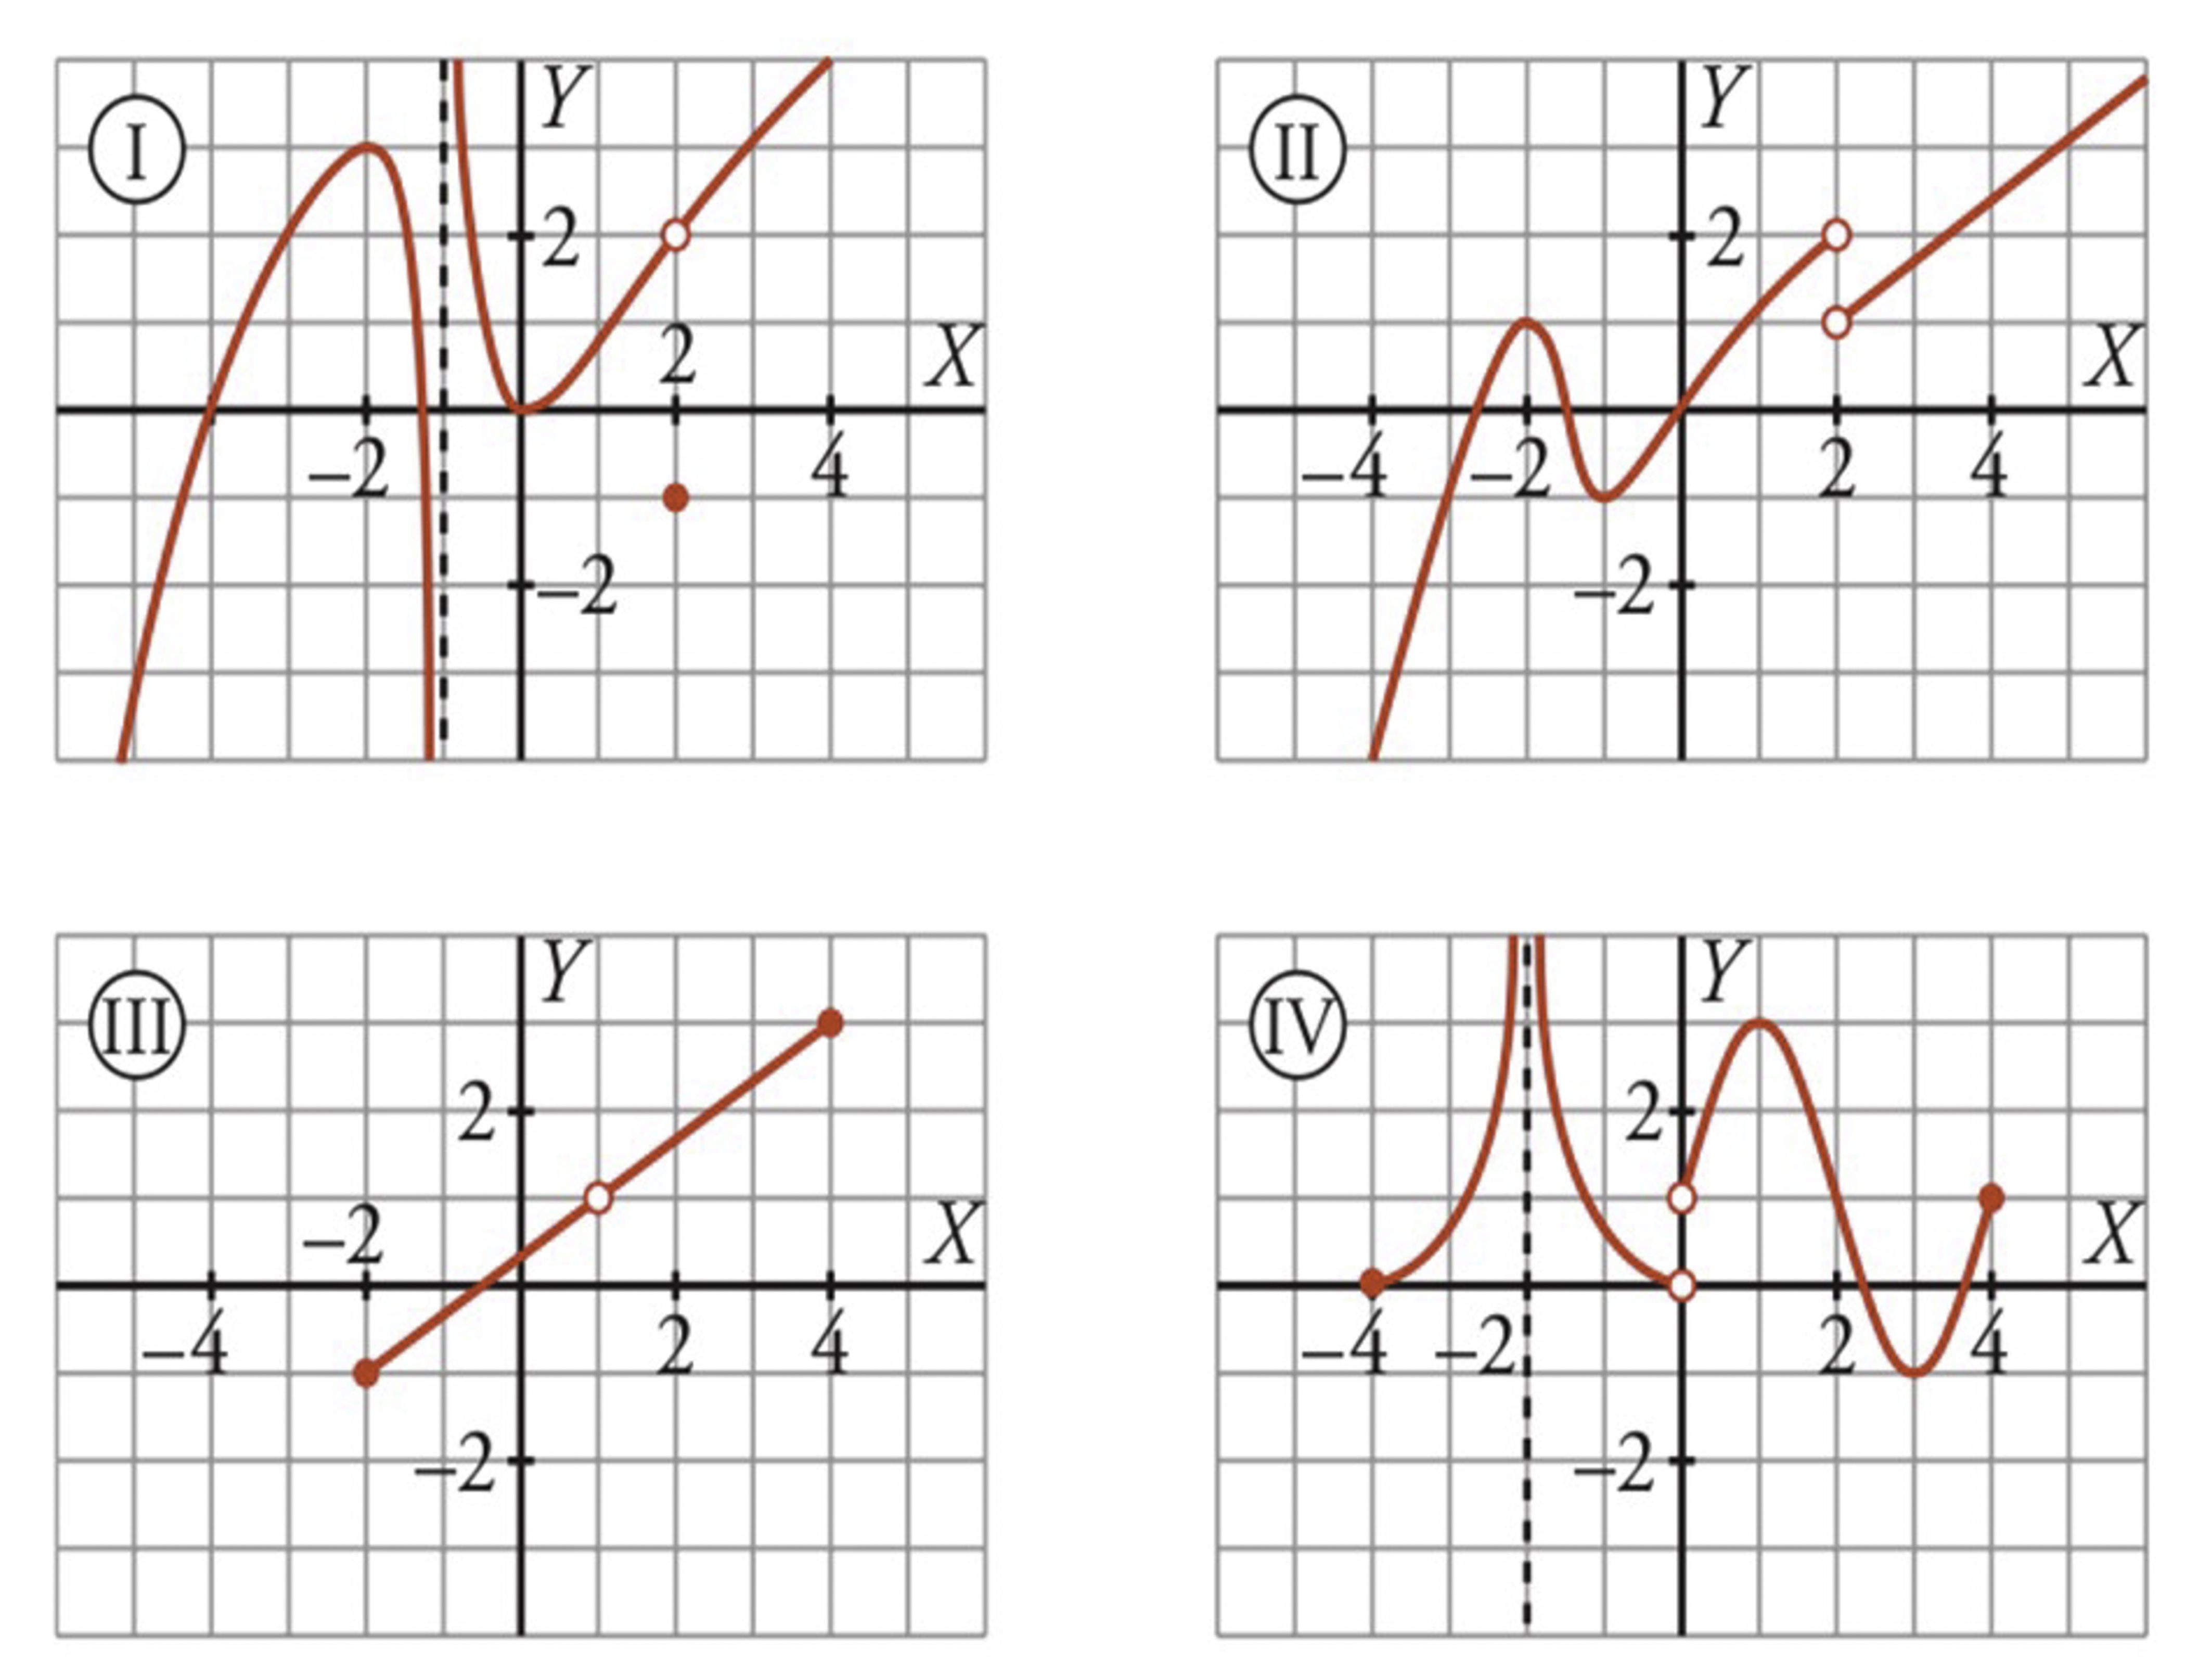
\includegraphics[width=0.8\textwidth]{tp2_fig14.jpg} 
\end{center}

\fbox{ \parbox{0.98\linewidth}{
\noindent
\begin{mydef} \textbf{Funciones compuestas.}\\
Dadas dos funciones $f$ y $g$ , se define como la \textbf{composición} de la función $f$ con la función $g$ , a la función denotada $f \circ g$ ( que se lee  $f$ compuesta con $g$ ), cuya regla de correspondencia es:
\begin{equation*}
f  \circ g = f(g(x))
\end{equation*}
cuyo dominio está representado por el conjunto:
\begin{center} 
Dom $(f \circ g) = \{ x  \in Dom(g) / g(x) \in Dom(f)\} $\\
\end{center}
\end{mydef}
}}

\vspace{0.5 cm}
Para obtener la regla de correspondencia de la función $f \circ g$ según la definición anterior, basta con sustituir la función $g(x)$ en la variable independiente de la función $f$ .\\
Así por ejemplo, sean las funciones $f(x) = 4x^2 -1$ y $g(x) =\sqrt{x}$, entonces, la función compuesta $f \circ g$  es:\\
\begin{equation*}
f  \circ g = f(g(x)) = 4.(g(x))^2-1 = 4.(\sqrt{x})^2-1 = 4|x|-1
\end{equation*}

Para obtener la función compuesta $g \circ f$  debemos sustituir por $f(x)$ a la variable de $g$. Utilizando las mismas funciones del ejemplo anterior,  la función compuesta $g \circ f$  es:
\begin{equation*}
g  \circ f = g(f(x)) = \sqrt{f(x)} = \sqrt{4x^2-1}
\end{equation*}
%\vspace{0.2 cm}

%28
\item 	Dadas las funciones $f(x) = \frac{1}{2}x -1$, $g(x) = x^2-1$ y $h(x) = \frac{1}{x-1}+2$, calcular:
\begin{multicols}{4}
\begin{enumerate} [leftmargin=2cm]
\item$f \circ g$ 
\item $f \circ h$
\item$g \circ f$
\item  $g \circ h$
\end{enumerate}
\end{multicols}

%29
\item Sean  $f(x) = 2x-3 $ y $g(x) =\frac{3}{x-2} +2$, hallar las funciones compuestas $f \circ g$  y $g \circ f$, y el dominio de ambas composiciones. Graficarlas (usar el Graph 4.3).

%30
\item Dadas las funciones $f(x) = ax-2$ y $g(x) =\frac{x-3}{2x-1}$, hallar el valor de $a$ para que  $(g \circ f) (2) = 0$



\end{enumerate}

\end{document}
